\documentclass[11pt,french,french]{article}
\usepackage{lmodern}
\usepackage{amssymb,amsmath}
\usepackage{ifxetex,ifluatex}
\usepackage{fixltx2e} % provides \textsubscript
\ifnum 0\ifxetex 1\fi\ifluatex 1\fi=0 % if pdftex
  \usepackage[T1]{fontenc}
  \usepackage[utf8]{inputenc}
\else % if luatex or xelatex
  \ifxetex
    \usepackage{mathspec}
    \usepackage{xltxtra,xunicode}
  \else
    \usepackage{fontspec}
  \fi
  \defaultfontfeatures{Mapping=tex-text,Scale=MatchLowercase}
  \newcommand{\euro}{€}
\fi
% use upquote if available, for straight quotes in verbatim environments
\IfFileExists{upquote.sty}{\usepackage{upquote}}{}
% use microtype if available
\IfFileExists{microtype.sty}{%
\usepackage{microtype}
\UseMicrotypeSet[protrusion]{basicmath} % disable protrusion for tt fonts
}{}
\usepackage[margin=0.90in]{geometry}
\ifxetex
  \usepackage{polyglossia}
  \setmainlanguage{}
\else
  \usepackage[shorthands=off,french]{babel}
\fi
\usepackage{longtable,booktabs}
\ifxetex
  \usepackage[setpagesize=false, % page size defined by xetex
              unicode=false, % unicode breaks when used with xetex
              xetex]{hyperref}
\else
  \usepackage[unicode=true]{hyperref}
\fi
\hypersetup{breaklinks=true,
            bookmarks=true,
            pdfauthor={},
            pdftitle={},
            colorlinks=true,
            citecolor=blue,
            urlcolor=blue,
            linkcolor=magenta,
            pdfborder={0 0 0}}
\urlstyle{same}  % don't use monospace font for urls
\setlength{\parindent}{0pt}
\setlength{\parskip}{6pt plus 2pt minus 1pt}
\setlength{\emergencystretch}{3em}  % prevent overfull lines
\setcounter{secnumdepth}{5}

\providecommand{\tightlist}{%
  %\setlength{\itemsep}{0pt}
  \setlength{\parskip}{0pt}
  }

%%% Use protect on footnotes to avoid problems with footnotes in titles
\let\rmarkdownfootnote\footnote%
\def\footnote{\protect\rmarkdownfootnote}


  \title{~\emph{Word-Embedding} et sentiments des ménages avec Twitter}
    \author{Kim Antunez, Romain Lesauvage, Alain Quartier-la-Tente\\
sous l'encadrement de Benjamin Muller (Inria)}
    \date{}
  
\usepackage{caption}
\usepackage{graphicx}
\usepackage{natbib}
\usepackage[dvipsnames]{xcolor}
\usepackage{fontawesome5}
\DeclareMathOperator{\arctanh}{arctanh}
\usepackage{subcaption}
\usepackage{amsfonts}
\usepackage{dsfont}
\usepackage{xspace}
\usepackage{enumitem}
\usepackage{pifont}
\usepackage{wrapfig}
\usepackage{textpos}
\usepackage{array}


\usepackage[tikz]{bclogo}
\newcounter{comptEncadre}
\renewcommand\thecomptEncadre{%\thesection.
\arabic{comptEncadre}}
\definecolor{processblue}{cmyk}{0.96,0,0,0}
\newenvironment{encadre}[2][false]{\refstepcounter{comptEncadre}
      %\addcontentsline{exp}{encadres}{\protect\numberline{\thecomptEncadre}#1}%
\begin{bclogo}[couleur=processblue!5,arrondi=0.1,
logo=\bcloupe,barre=none,couleurBord=blue!60!green,nobreak = #1]{ {\sc \textbf{Encadré \thecomptEncadre}} -  #2}
\smallskip
}{\end{bclogo}}

\begin{document}

\maketitle


{
\hypersetup{linkcolor=black}
\setcounter{tocdepth}{2}
\tableofcontents
}
\begin{textblock*}{\textwidth}(0cm,-21cm)
\begin{center}

\includegraphics[height=2.5cm]{img/LOGO-ENSAE.png}
\end{center}
\end{textblock*}

\begin{textblock*}{\textwidth}(0cm,2.5cm)
\begin{center}
\begin{minipage}{0.7\textwidth}

\begin{wrapfigure}{L}{0cm}

\includegraphics[height=0.8cm]{img/avatars.png}
\end{wrapfigure}

$\phantom{saut}$

\emph{Retrouvez l'ensemble du projet et son code sur}

https://github.com/ARKEnsae/TweetEmbedding

\end{minipage}
\end{center}

\end{textblock*}

\newpage 

\section*{Introduction}\label{introduction}
\addcontentsline{toc}{section}{Introduction}

Grâce à l'évolution des méthodes d'apprentissage profond (\emph{Deep
Learning}), l'appréhension du langage naturel est aujourd'hui devenue
une discipline à part entière (\emph{Natural Language Processing}). Ce
succès s'explique en partie grâce à l'émergence de techniques non
supervisées d'apprentissage de représentation de structures
linguistiques. Les méthodes de \emph{word-embedding} («~plongement
lexical~» en français) permettent de représenter chaque mot d'un
dictionnaire par un vecteur de nombres réels afin que les mots qui
apparaissent dans des contextes similaires possèdent des vecteurs
correspondants qui sont relativement proches (au sens d'une distance
définie). Les variantes du modèle \emph{word2vec}, développé par une
équipe de recherche chez Google (\cite{Mikolov}), sont parmi les plus
célèbres et sont ceux sur lesquels se concentrera notre projet.

Dans ce projet de statistique appliquée, nous étudierons dans un premier
temps en détail et implémenterons le modèle \emph{word2vec} (partie
\ref{sec:word2vec}). Dans un deuxième temps, nous évaluerons le modèle
implémenté et l'appliquerons sur une base de données composée d'1,3
million de tweets publiés en France entre 2013 et 2017 (partie
\ref{sec:evaluation}). Enfin, nous mobiliserons des techniques d'analyse
de sentiment afin de créer des indicateurs qui pourront être comparés
aux indicateurs produits dans la statistique publique, en particulier
concernant l'opinion des ménages (partie \ref{sec:sentimentalAnalysis}).

La figure \ref{fig:schemaRecap} résume l'ensemble de notre démarche.

\vspace{2cm}

\begin{figure}[!htb]
\tikzstyle{myboxnorm} = [very thick,
    rectangle, rounded corners, inner sep=2pt, inner ysep=3pt, right,
    align=center]
\tikzstyle{myboxw2v} = [draw=red!50, fill=orange!10, myboxnorm]
\tikzstyle{myboxmod} = [draw=blue!60!green, fill=blue!5, myboxnorm]
\tikzstyle{myboxcomp} = [draw=green!50!black, fill=green!5, myboxnorm]

\tikzstyle{titlenorm} = [fill=white, very thick,
    rectangle, inner sep=2pt, inner ysep=2pt,font=\bfseries,
    text width=4.2cm, above=-0.3cm, align=center,
    minimum height=1.15cm]
\tikzstyle{titlew2v} = [draw=red!50, text = red!50,titlenorm]
\tikzstyle{titlemod} = [draw=blue!60!green,text=blue!60!green,titlenorm]
\tikzstyle{titlecomp} = [draw=green!50!black,text=green!50!black, titlenorm]    

\tikzstyle{fleche} = [->,rounded corners,line width=1pt]

\begin{tikzpicture}
\usetikzlibrary{fit}
\usetikzlibrary{arrows.meta}
%Il faut d'abord faire les boites
% w2vec
\node[fit={(2.5,1.5) (-3.,-3.5)}, myboxw2v,semitransparent] (w2vrect) {};
\node[fit={(2.7,1.5) (8.2,-5.5)}, myboxmod,semitransparent] (rectmod) {};
\node[fit={(13.9,1.5) (8.4,-5.5) }, myboxcomp,semitransparent] (rectcomp) {};

\node at (0,0) [myboxw2v] (tweets) {Tweets};
\node at (2.4,0) [myboxw2v] (we) {\textit{word-embedding}};
% sentiment
\node at (0,-4.5) [myboxnorm,text width=2.5cm, draw = black] (bddsent) {Échantillon de tweets annotés
};

% analyse de sentimentsentiment
\node at (7,0) [myboxmod] (logit) {Modèle logit};
\node at (7,-4.5) [myboxmod,text width=2.22cm] (baseline) {Modèle lexical};

% analyse de sentimentsentiment
\node at (12,0) [myboxcomp,text width=3.8cm] (indsent) {Indices mensuels de \\sentiment des tweets};

\node at (12,-4.5) [myboxcomp,text width=3.8cm] (camme) {Indicateur synthétique \\de confiance des

ménages (Insee)};

%Fleches
\draw[fleche] (tweets.east) --(we.west) node[below = 0.2cm,pos=1]{
\begin{minipage}{5cm} \footnotesize
  \begin{itemize}[label=\scalebox{.6}{\ding{110}}] 
  \item tokénisation
  \item choix hyperparamètres
  \item évaluation : 
  \begin{itemize}[label=\scalebox{.6}{\ding{117}}]
    \item similarité cosinus
    \item réduction de dimension (ACP/TSNE)
    \item jugement humain
  \end{itemize}
  \end{itemize} 
\end{minipage} 
};
\draw[fleche] (bddsent.east)--(baseline.west) 
  node[pos=0.36,text width=3cm]{
    \footnotesize bases  
    
    test/entraînement}
  node[pos=0.96, below = 0.05cm,text width=2.5cm]{
    \footnotesize sentiment 
    
    moyen d'un mot};
\draw[fleche] (bddsent.east)--++(2,0)--++(0,0.8)-|(logit.south);
\draw[fleche] (we.east)--(logit.west)node[pos=0.89,text width=2.5cm]{\footnotesize \emph{sentence}
  
  \emph{embedding}};
\draw[fleche] (logit.east)--
  (indsent.west)node[pos=0.62,text width=2.5cm]{\footnotesize moyennes
  
  mensuelles};
\draw[fleche] (baseline.east)-|(9.6,0)--(indsent.west);
\draw[fleche,<->] (indsent.south)--(camme.north) 
  node[pos=.5,text width=2.5cm, right=0.2cm]{\footnotesize distance entre
  
  indicateurs}
  node[pos=.5,text width=1.7cm, left]{\footnotesize prévision /
  
  causalité};

\node[titlew2v] at (w2vrect.north) { word2vec \\
(skip-gram)};
\node[titlemod] at (rectmod.north) { Analyse de \\
sentiment d'un tweet};
\node[titlecomp] at (rectcomp.north) { Comparaison \\
d'indices mensuels};
\end{tikzpicture}
\captionsetup{margin=0cm,format=hang,justification=justified}
\caption{Synthèse de notre démarche : construire un indice mensuel de sentiment à partir de tweets.}\label{fig:schemaRecap}
\end{figure}

\newpage

\section{\texorpdfstring{Implémentation du modèle
\emph{word2vec}}{Implémentation du modèle word2vec}}\label{sec:word2vec}

\subsection{\texorpdfstring{Le modèle \emph{word2vec}, un modèle de
\emph{word-embedding}}{Le modèle word2vec, un modèle de word-embedding}}\label{le-moduxe8le-word2vec-un-moduxe8le-de-word-embedding}

Le \emph{Natural Language Processing} (NLP ou «~traitement automatique
du langage naturel~») est une branche du \emph{machine learning} visant
à analyser, traiter et reproduire le langage humain. Les différentes
variantes du modèle de NLP \emph{word2vec}, développé par une équipe de
recherche chez Google (\cite{Mikolov}), sont parmi les plus célèbres et
utilisent le \emph{word-embedding} --- plongement lexical en français.

\subsubsection{\texorpdfstring{Historique : de la sémantique vectorielle
à
\emph{word2vec}}{Historique : de la sémantique vectorielle à word2vec}}\label{historique-de-la-suxe9mantique-vectorielle-uxe0-word2vec}

La «~sémantique vectorielle~» est née dans les années 1950\footnote{L'ouvrage
  \cite{Jurafsky} permet de retracer avec une grande richesse
  l'évolution des méthodes de NLP.}. Il s'agit d'une méthode algébrique
de représentation d'un document visant à réaliser des tâches diverses
(détecter le plagiat, filtrer des articles\dots). Il est alors
nécessaire de capter de nombreux types de proximité entre mots : les
synonymes (automobile / voiture), antonymes (froid / chaud),
connotations positives \emph{versus} négatives (heureux / triste), etc.

Un modèle répondant à toutes ces exigences ne peut exister. Pour y
répondre au mieux, la sémantique vectorielle puise son inspiration des
travaux linguistiques des années 1950 et en particulier de
l'~«~hypothèse de distribution~» selon laquelle un mot se définit par
son environnement. Dit autrement : les mots qui se produisent dans un
contexte identique tendent à avoir des significations
similaires\footnote{Comme l'a écrit le linguiste britannique John Rupert
  Firth en 1957, «~Vous connaîtrez un mot par ses fréquentations~».}.

Les premiers modèles sémantiques (comme le \emph{term frequency-inverse
document frequency} (TF-IDF)) représentaient les relations entre mots
grâce à des très grandes matrices, dites \emph{sparses}, dont les
dimensions correspondaient à la taille du vocabulaire (contenant donc
beaucoup de 0). Les méthodes de \emph{word-embedding} qui sont ensuite
apparues ont permis de représenter chaque mot d'un dictionnaire par un
vecteur de nombres réels dense (peu de 0) de plus faible dimension (en
général entre 50 et 1000). Si la réduction de dimension rend les
vecteurs-mots moins facilement interprétables, elle a pour grand
avantage de faciliter et d'accélérer les tâches d'apprentissage
impliquant ces mots.

\cite{Mikolov} ont mis en avant en 2013 les méthodes de
\emph{word-embedding} à travers la création de \emph{word2vec}. Ce
modèle de réseaux de neurones\footnote{C'est l'article \cite{Bengio} qui
  a introduit dix ans avant \emph{word2vec} le premier modèle
  d'apprentissage de représentation de vecteurs-mots à partir d'un
  réseau de neurone simple.} à deux couches est rapidement devenu une
référence grâce à la grande précision des résultats qu'il permet
d'obtenir, pouvant être entraîné en un temps record sur un corpus très
volumineux.

\subsubsection{\texorpdfstring{\emph{word2vec}, un modèle
d'apprentissage
«~auto-supervisé~»}{word2vec, un modèle d'apprentissage «~auto-supervisé~»}}\label{subsec:word2vec}

En sortie du modèle \emph{word2vec}, chaque mot est représenté par un
vecteur dont la dimension est fixée par la valeur d'un hyperparamètre.
Les mots qui apparaissent dans des contextes similaires («~bonjour~» et
«~salut~» par exemple) seront représentés par des vecteurs relativement
proches dans l'espace vectoriel de définition de ces vecteurs. Dans la
même logique, \emph{word2vec} permet également de réaliser des
opérations vectorielles, comme dans l'exemple suivant souvent cité :
\(\overrightarrow{Paris} - \overrightarrow{France} + \overrightarrow{Italie} = \overrightarrow{Rome}\)
qui provient de \cite{Mikolov}.

Deux architectures du modèle \emph{word2vec} existent (graphique
\ref{fig:cbowskipgram}) :

\begin{itemize}
\item
  L'approche \emph{Continuous bags of words} dont l'objectif est
  d'estimer la probabilité d'observer un mot, appelé \textbf{«~focus~»},
  sachant le contexte dans lequel il apparaît (i.e. : les mots
  \textbf{voisins} qualifiés de \textbf{«~contextes~»}).
\item
  L'approche \emph{Skip-gram} a un objectif inverse : estimer, pour
  chaque mot du vocabulaire, la probabilité d'être proche du mot focus.
  C'est cette approche que nous étudions dans ce projet et dans la suite
  de ce rapport. 
\end{itemize}

\begin{figure}[htp]
\begin{center}
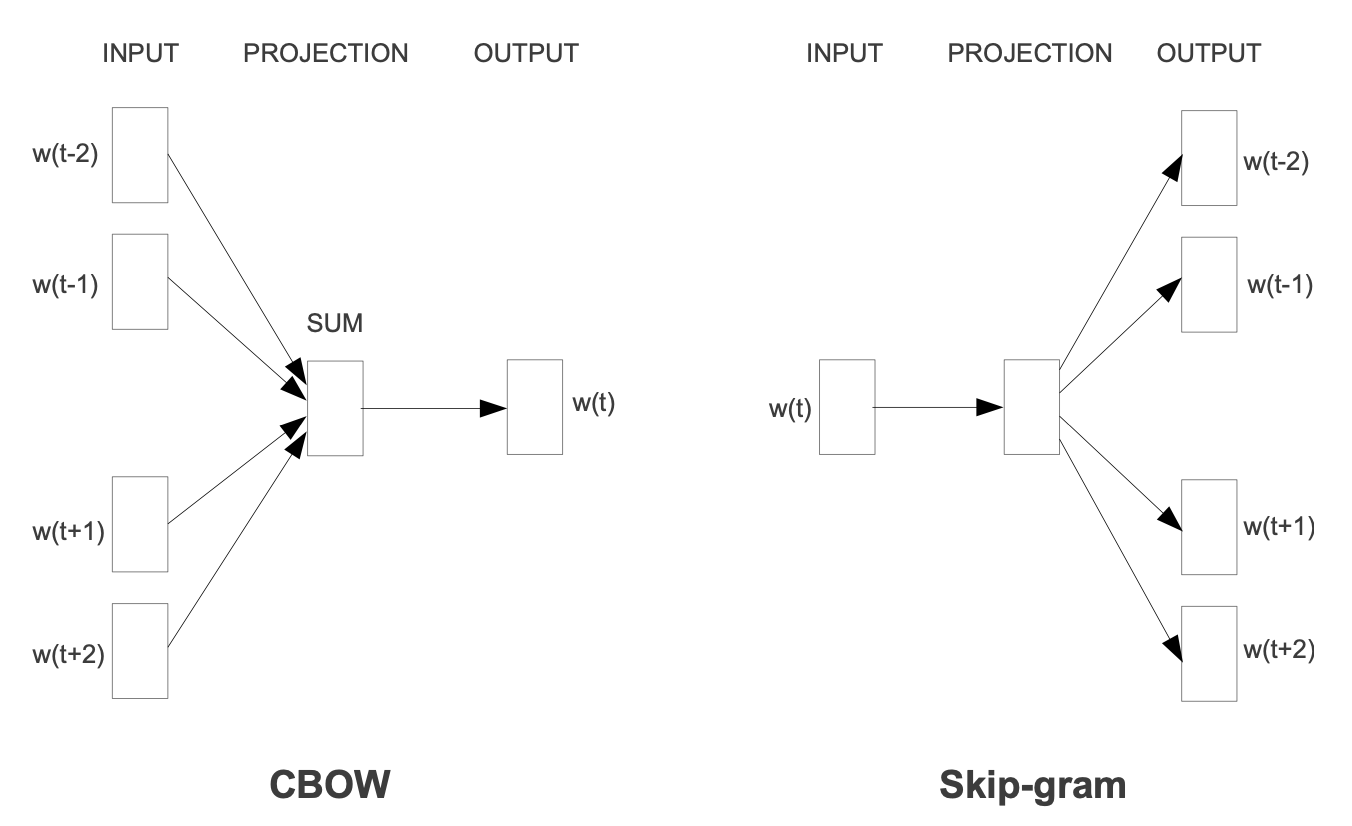
\includegraphics[width=.6\textwidth]{img/cbow_skip_gram.png}
\end{center}
\captionsetup{margin=0cm,format=hang,justification=justified}
\caption{Architecture des modèles *Continuous bags of words* (CBOW) et *Skip-gram*.}\label{fig:cbowskipgram}
%\vspace{-0.3cm}
\footnotesize
\emph{Source : \cite{Mikolov}}
\end{figure}

Pour transformer chaque mot en un vecteur, au lieu de simplement compter
les fréquences d'apparition des mots contextes voisins d'un mot
focus\footnote{Comme dans les premiers modèles sémantiques dits
  \emph{sparses}.}, nous entraînons un réseau de neurones sur une tâche
annexe : on construit un classifieur dont la tâche de prédiction est
binaire pour chacun des mots du vocabulaire et répond à la question
(dans le cas \emph{Skip-gram}) «~Est-ce que ce mot contexte est
susceptible d'être voisin du mot focus ?~». Ce n'est pas la prédiction
en elle-même qui nous intéresse, mais plutôt le poids du classifieur en
sortie du modèle qui correspondra aux \emph{word-embeddings}.

Les voisins d'un mot focus reposent sur un hyperparamètre : la fenêtre
(\emph{window} ou \(w\)). Pour \(w = p\), les voisins du mot focus sont
les \(p\) mots précédents et les \(p\) mots suivants dans la phrase. Par
exemple, dans la phrase :

\begin{quote}
\LARGE \textbf{``}\normalsize \emph{Le professeur de statistique est strict avec ses élèves.} \LARGE \textbf{''}\normalsize
\end{quote}

pour \(w=2\), si le mot focus est «~statistique~» alors le contexte qui
lui est associé est : \texttt{{[}professeur,\ de,\ est,\ strict{]}} ; si
le mot focus est «~professeur~» alors le contexte qui lui est associé
est : \texttt{{[}Le,\ de,\ statistique{]}}.

Pour déterminer les représentations vectorielles des mots, nous
entraînons le réseau de neurones en le nourrissant des paires
\texttt{{[}focus,\ contexte{]}}\footnote{Dans notre exemple :
  \texttt{{[}statistique,\ professeur{]},\ {[}statistique,\ de{]}}\dots}
contenues dans les différentes phrases (ici tweets) du corpus afin qu'il
puisse déterminer les probabilités d'apparition d'un mot dans le
voisinage d'un autre mot (voir description de l'algorithme en partie
\ref{sec:skipgram}).

Ainsi, la grande force du modèle d'apprentissage \emph{word2vec} est
qu'il est «~auto-supervisé~». En effet, comme nous avons vu plus haut,
le corpus est considéré comme une donnée d'entraînement implicitement
supervisée, ce qui nous évite d'avoir à mobiliser des corpus annexes
annotés.

\subsection{\texorpdfstring{L'algorithme
\emph{Skip-gram}}{L'algorithme Skip-gram}}\label{sec:skipgram}

L'objectif de cette partie est de décrire le fonctionnement de
l'approche \emph{Skip-gram}.

Dans la suite de ce projet nous noterons \(n\) la taille du vocabulaire
(i.e. : le nombre de mots différents utilisés dans les tweets) et
\(dim\) la dimension retenue pour les \emph{word-embeddings}. Comme
décrit dans la partie \ref{subsec:word2vec}, l'approche \emph{Skip-gram}
peut être vue comme un réseau de neurones à deux couches avec :

\begin{itemize}
\item
  En entrée une matrice \(W_e\) de taille \(n\times dim\) ;
\item
  En sortie une matrice \(W_s\) de taille \(n\times dim\).
\end{itemize}

Ces deux matrices sont initialisées en générant des lois normales
\(\mathcal N(0,1)\). Elles sont ensuite mises à jour, grâce aux couples
\texttt{{[}focus,\ contexte{]}} construits à partir du corpus (partie
\ref{subsec:baseentrainement}), par un algorithme de descente de
gradient. À la fin de l'algorithme, ce sont ces matrices qui donneront
la représentation vectorielle des mots du vocabulaire. Ainsi, la ligne
\(i\) de la matrice \(W=\frac{W_e+W_s}{2}\) donnera la représentation du
\(i\)\textsuperscript{ème} mot du vocabulaire en dimension \(dim\).

\subsubsection{Construction de la base
d'entraînement}\label{subsec:baseentrainement}

Peu de traitements sont effectués sur la base initiale : nous mettons
tout en minuscule, remplaçons les ponctuations par des espaces, mais
laissons tous les chiffres et les accents. Chaque phrase\footnote{Dans
  notre cas une phrase correspond à un tweet, même si ce tweet peut être
  composé de plusieurs phrases.} est ensuite \emph{tokénisée} par la
chaîne de caractères correspondant à un espace \texttt{"\ "} : on
considère qu'il y a autant de mots de que chaînes de caractères séparées
par un espace\footnote{Les mots composés sont donc considérés comme
  plusieurs mots distincts.}. Par exemple, la phrase :

\begin{quote}
\LARGE \textbf{``}\normalsize \emph{Que pensez-vous de CE projet?(i.e. : qu'avez-vous retenu en 10min ?)} \LARGE \textbf{''}\normalsize
\end{quote}

est décomposée en 14 mots
\texttt{{[}que,\ pensez,\ vous,\ de,\ ce,\ projet,\ i,\ e,\ qu,\ avez,\ vous,\ retenu,\ en,\ 10min{]}}.

Nous effectuons enfin un traitement sur les mots rares. Si un mot
apparaît strictement moins de 10 fois, nous lui affectons la valeur
«~lowfrequency~»\footnote{Dans le corpus de tweets que nous utiliserons
  ultérieurement, un mot rare apparaît moins de 10 fois sur les 31 400
  000 mots utilisés dans le corpus. Rassembler les mots rares permettra
  de passer d'un vocabulaire d'environ 635 000 mots à 70 000 mots en
  réduisant le nombre de mots de seulement 3,0 \%.}.

Comme décrit dans la partie \ref{subsec:word2vec}, les couples
\texttt{{[}focus,\ contexte{]}} dépendent d'un hyperparamètre : la
fenêtre \(w\). Pour éviter que les mots trop fréquents, souvent peu
informatifs (comme les pronoms personnels), soient sur-entraînés, deux
traitements sont effectués :

\begin{enumerate}
\def\labelenumi{\arabic{enumi}.}
\item
  Pour chaque phrase on effectue un sous-échantillonnage
  (\emph{subsampling}). Pour chaque mot \(w_i\) on note \(z(w_i)\) la
  proportion d'apparition de ce mot, c'est-à-dire le rapport entre le
  nombre de fois que ce mot apparaît et le nombre total de mots. La
  probabilité de garder le mot \(w_i\) est donnée par : \[
  \mathbb P(w_i) = \min\left\{\left(1+\sqrt{\frac{z(w_i)}{q}}  \right)
  \times
  \frac{q}{z(w_i)},1\right\}
  \] Le paramètre \(q\) appelé «~sample~» --- échantillonnage ---
  contrôle le nombre de mots sous-échantillonnés (plus il est grand,
  plus la probabilité de garder le mot \(w_i\) est grande). Si \(q\)
  vaut 0,001 (valeur par défaut) alors par exemple :

  \begin{itemize}
  \tightlist
  \item
    \(\mathbb P(w_i) = 1\) (\(w_i\) est toujours gardé) lorsque
    \(z(w_i)\leq 0,0026\), c'est-à-dire si \(w_i\) représente moins de
    0,26 \% du nombre total de mots.\\
  \item
    \(\mathbb P(w_i) = 0,5\) (50 \% de chance de garder \(w_i\)) lorsque
    \(z(w_i)=0,00746\).\\
  \item
    \(\mathbb P(w_i) = 0,033\) (3,3 \% chance de garder \(w_i\)) lorsque
    \(z(w_i)=1,0\) (si le corpus n'est constitué que du mot \(w_i\), ce
    qui serait bien sûr absurde).
  \end{itemize}
\end{enumerate}

Ce sous-échantillonnage est effectué de manière indépendante pour chaque
phrase : un même mot peut donc être sous-échantillonné dans une phrase
et ne pas l'être dans une autre.

\begin{enumerate}
\def\labelenumi{\arabic{enumi}.}
\setcounter{enumi}{1}
\tightlist
\item
  Pour chaque phrase, on tire au hasard (selon une loi uniforme) un mot
  focus, pour lequel on tire un mot \emph{contexte} au hasard dans la
  fenêtre \(w\), en imposant que les deux mots choisis soient parmi les
  mots sous-échantillonnés\footnote{Si pour une phrase, aucun couple
    \texttt{{[}focus,\ contexte{]}} ne figure simultanément dans les
    mots sous-échantillonnés, alors aucun couple n'est retenu pour cette
    phrase.}. Par exemple, nous supposons que dans la phrase
  \texttt{{[}que,\ pensez,\ vous,\ de,\ ce,\ projet,\ i,\ e,\ qu,\ avez,\ vous,\ retenu,\ en,\ 10min{]}},
  les mots sous-échantillonnés sont les mots en positions 2, 5, 6, 8, 9,
  10, 11, 12, 13 et 14. Pour mieux comprendre, nous remplaçons les mots
  non échantillonnés par «~nonsubsampled~». La phrase devient alors
  \texttt{{[}nonsubsampled,\ pensez,\ nonsubsampled,\ nonsubsampled,\ ce,\ projet,\ nonsubsampled,\ e,\ qu,\ avez,\ vous,\ retenu,\ en,\ 10min{]}}.
  Si \(w=2\) alors le mot focus tiré ne peut pas être «~pensez~» puisque
  dans ce cas il n'y aurait aucun mot contexte associé. Si le mot focus
  tiré est «~qu~» alors le mot contexte est tiré au hasard parmi
  \texttt{{[}e,\ avez,\ vous{]}}.
\end{enumerate}

Ce mécanisme va être répété sur toutes les phrases du corpus et
l'ensemble du corpus va être parcouru plusieurs fois. Le nombre de fois
que l'ensemble du corpus est parcouru est appelé \emph{epochs}.

\subsubsection{Descente de gradient}\label{subsec:descentedegradient}

Pour chaque couple \texttt{{[}focus,\ contexte{]}}, les matrices \(W_e\)
et \(W_s\) sont mises à jour par descente de gradient. C'est-à-dire que
les matrices \(\theta^{(t)} = W_e\) et \(\theta^{(t)} = W_s\) obtenues
après la \(t\)\textsuperscript{ème} itération de l'algorithme sont mises
à jour par l'équation : \[
\theta^{(t+1)} = \theta^{(t)} - \eta \nabla_\theta Loss(\theta^{(t)})
\] avec \(\eta\) le taux d'apprentissage (un hyperparamètre à fixer) et
\(Loss(\theta)\) la fonction de perte.

Le modèle \emph{word2vec} a initialement été construit en utilisant une
fonction de perte dérivée de la fonction \emph{softmax} (voir partie
\ref{subsec:softmax} et \cite{Mikolov}). L'algorithme a ensuite été
amélioré en utilisant le \emph{negative sampling} (voir partie
\ref{subsec:negsampling} et \cite{MikolovNS}).

\paragraph{Version softmax}\label{subsec:softmax}

Soit \(w_1,\,\dots,\,w_T\) les mots utilisés pour entraîner le modèle.
L'objectif du modèle \emph{Skip-gram} est, étant donné un mot focus, de
prévoir quels sont les mots voisins contextes dans une certaine fenêtre
\(w\). Mathématiquement, on cherche à maximiser la quantité :

\begin{equation}
\frac 1 T\sum_{t=1}^T\sum_{-w\leq j \leq w,\,j\ne 0} \log \mathbb P(w_{t+j}\vert w_{t})
\label{eq:objSoftMax}
\end{equation}

où :

\begin{itemize}
\item
  les \(w_{t+j}\) sont les mots voisins de \(w_t\) (\(w_t\) est donc un
  mot focus et \(w_{t+j}\) un mot contexte) ;
\item
  \(\mathbb P(w_{t+j}\vert w_{t})\) est la probabilité d'observer le mot
  contexte \(w_{t+j}\) sachant que l'on a observé le mot focus \(w_t\).
  Cette quantité est calculée en fonction des matrices \(W_e\) et
  \(W_s\) à partir de la fonction softmax \footnote{Étant donné le
    vecteur \(z=(z_1,\,\dots,\,z_n)\) la fonction softmax est la
    fonction qui à \(z\) associe le vecteur dont la
    \(j\)\textsuperscript{ème} coordonnée est égale à
    \(\frac{\exp(z_j)}{\sum_{i=1}^n\exp(z_i)}\).}. En notant \(n\) la
  taille du vocabulaire et \(W_{e,w_i}\) et \(W_{s,w_i}\) les
  représentations vectorielles du mot \(w_i\) respectivement dans la
  matrice d'entrée et de sortie, cette probabilité est égale à\footnote{Dans
    tout le rapport, nous utiliserons la notation \(^{t}X\) pour
    désigner la transposée de la matrice \(X\).} : \[
  \mathbb P(w_{contexte}\vert w_{focus}) = 
  \frac{
  \exp(W_{e,w_{focus}}\times {}^tW_{s,w_{contexte}})
  }{
  \sum_{i=1}^n\exp(W_{e,w_{focus}}\times {}^tW_{s,w_{i}})
  }
  \]
\end{itemize}

Maximiser l'équation \eqref{eq:objSoftMax} revient à minimiser la fonction
de perte suivante pour chaque couple \texttt{{[}focus,\ contexte{]}} :

\[
Loss_{1}=-\log\mathbb P(w_{contexte}\vert w_{focus}) =
-W_{e,w_{focus}}\times {}^tW_{s,w_{contexte}}+
\log\left(\sum_{i=1}^n\exp(W_{e,w_{focus}}\times {}^t W_{s,w_i})\right)
\] L'inconvénient de cette méthode est qu'elle est très gourmande en
temps de calcul. En effet, pour chaque couple
\texttt{{[}focus,\ contexte{]}}, la complexité du calcul de
\(\log\mathbb P(w_{contexte}\vert w_{focus})\) est proportionnelle à la
taille du vocabulaire. La taille du vocabulaire pouvant être très grande
(par exemple, dans notre base de tweets, cette taille est de 70 330), le
temps de calcul peut vite devenir très important.

C'est pourquoi la version \emph{softmax} est très peu utilisée dans les
implémentations de \emph{Skip-gram}. Une approche alternative, le
\emph{negative sampling} avec une fonction sigmoïde, moins gourmande en
temps de calcul, est alors souvent préférée\footnote{Une autre
  alternative à l'approche \emph{softmax} parfois utilisée est
  l'approche \emph{hierarchical softmax} qui se base sur l'utilisation
  d'arbres binaires de classification. La complexité de cet algorithme
  est proportionnelle à \(\log_2n\) mais reste plus importante que celle
  de l'approche \emph{negative sampling}.}.

\paragraph{\texorpdfstring{Version \emph{negative
sampling}}{Version negative sampling}}\label{subsec:negsampling}

Le \emph{negative sampling} est basé sur le concept du \emph{Noise
Contrastive Estimation} --- estimation contrastée du bruit --- où on
cherche, à partir d'un modèle logistique, à différencier un vrai signal
(un vrai couple \texttt{{[}focus,\ contexte{]}}) d'un faux (un bruit,
qui correspondrait à un faux couple \texttt{{[}focus,\ contexte{]}}
généré aléatoirement).

Dans cette approche, plutôt que de mettre à jour l'ensemble des
représentations vectorielles des mots pour chaque couple
\texttt{{[}focus,\ contexte{]}}, on tire \(K\) mots au hasard du
vocabulaire \((w_{neg,\,i})_{i=1..K}\), selon une loi \(P\) (définie
plus tard), en considérant que ces mots ne seront pas des mots voisins
de \texttt{focus}\footnote{Il est bien sûr possible que, parmi les mots
  tirés au hasard, il y ait des mots qui soient vraiment dans le
  contexte. Cependant, puisque la taille du vocabulaire est très grande,
  on considère que cette erreur est négligeable.}.

L'approche \emph{softmax} peut être vue comme un problème de
classification multiclasses : étant donné un mot \texttt{focus}, on
estime la probabilité que les autres mots soient parmi ses voisins
(chaque classe étant un mot du vocabulaire). L'idée du \emph{negative
sampling} est de transformer ce problème de classification multiclasses
en un problème de classification binaire d'une variable \(D\) : pour
chaque couple \texttt{{[}focus,\ mot2{]}}, on cherche à déterminer si
\texttt{mot2} est dans le contexte de \texttt{focus}. Si c'est le cas,
alors \(D=1\) (\texttt{mot2} est positif et est le \texttt{contexte}),
sinon \(D=0\) (\texttt{mot2} est négatif, il appartient à
\((w_{neg,\,i})_{i=1..K}\)).

On cherche donc à maximiser
\(\mathbb P(D=1\vert w_{focus},w_{contexte})\) et
\(\mathbb P(D=0\vert w_{focus},w_{neg,\,i})\). Pour estimer ces
probabilités, on utilise une fonction sigmoïde plutôt que la fonction
softmax : \[
\mathbb P(D=1\vert w_{focus},w_{contexte})=\sigma(W_{e,w_{focus}}{}^tW_{s,w_{contexte}}) = 
\frac{1}{1+\exp(-W_{e,w_{focus}}{}^tW_{s,w_{contexte}})}
\] et : \[
\mathbb P(D=0\vert w_{focus},w_{neg,\,i})=\sigma(-W_{e,w_{focus}}{}^tW_{s,w_{neg,\,i}}) = 
\frac{1}{1+\exp(W_{e,w_{focus}}{}^tW_{s,w_{neg,\,i}})}
\] Par rapport à l'approche \emph{softmax}, on cherche toujours à
maximiser la quantité de l'équation \eqref{eq:objSoftMax} mais en estimant
\(\log\mathbb P(w_{contexte}\vert w_{focus})\) par : \[
\log\mathbb P(w_{contexte}\vert w_{focus}) =
\log\underbrace{\sigma (W_{e,w_{focus}}{}^tW_{s,w_{contexte}})}_{
\mathbb P(D=1\vert w_{focus},w_{contexte})
}+
\sum_{i=1}^K\mathbb E_{w_{neg,i}\sim P}[
\log
\underbrace{\sigma (-W_{e,w_{focus}}{}^tW_{s,w_{neg,\,i}})}_{
\mathbb P(D=0\vert w_{focus},w_{neg,\,i})
}
]
\]

Ainsi, pour chaque couple \texttt{{[}focus,\ contexte{]}} et un ensemble
\((w_{neg,\,i})_{i=1..K}\) de mots négatifs tirés, on associe la
fonction de perte suivante, à minimiser : \[
Loss_{2}=-\log\sigma (W_{e,w_{focus}}{}^tW_{s,w_{contexte}})
-
\sum_{i=1}^K
\log
\sigma (-W_{e,w_{focus}}{}^tW_{s,w_{neg,\,i}})
\] La complexité est ici bien plus faible que pour la fonction softmax
puisqu'elle est proportionnelle à \(K\).

\cite{MikolovNS} trouvent, empiriquement, que la meilleure distribution
\(P\) pour générer les mots négatifs est telle que : \[
\mathbb P_P(w_i) = \frac{z(w_i)^{3/4}}{
\sum_{j=1}^n z(w_j)^{3/4}
}
\] avec \(z(w_i)\) la fréquence d'apparition du mot \(w_i\).

Ils recommandent également de prendre \(K\in\{5,\dots,20\}\) pour les
petites bases de données et \(K\in\{2,\dots,5\}\) pour les grandes bases
de données. Dans ce projet, nous utiliserons \(K=5\) : pour chaque
couple \texttt{{[}focus,\ contexte{]}} nous tirons donc 5 mots négatifs.

\section{Évaluation du modèle implémenté}\label{sec:evaluation}

Malgré l'utilisation généralisée des \emph{word-embeddings}, très peu de
travaux théoriques expliquent ce qui est réellement capturé par ces
représentations de mots. C'est pourquoi ce modèle est principalement
évalué à l'aide de méthodes empiriques. L'annexe
\ref{annexe:commentEvaluer} décrit plus précisément les méthodes que
nous avons retenues pour évaluer la qualité des vecteurs-mots : la
similarité cosinus entre deux mots, la réduction de dimension de
l'espace des vecteurs-mots (ACP, t-SNE) et l'évaluation par jugement
humain.

\subsection{Évaluation sur un corpus fictif}\label{sec:corpusFictif}

Avant de nous attaquer au jeu de données complet décrit dans la partie
\ref{sec:hyperparametres}, nous avons évalué notre modèle sur un corpus
fictif afin de nous assurer de sa robustesse et de sa validité.

Nous générons tout d'abord 10 groupes de mots, chacun composé d'un
couple de référence de mots proches (du type
\texttt{{[}grand,\ petit{]}}) et de 10 autres mots que l'on considère
comme des mots appartenant au contexte des 2 mots «~référence~»
(\texttt{{[}taille,\ xl...{]}}).

Nous construisons ensuite un corpus fictif formé de 10 000 phrases de 9
mots de la manière suivante :

\begin{itemize}
\tightlist
\item
  on tire au hasard 1 des 10 groupes de mots ;
\item
  au sein de ce groupe, on tire au hasard 1 des 2 mots «~référence~» et
  5 des 10 mots contextes associés ;
\item
  on tire 3 mots «~bruits~» au hasard, parmi une liste 100 mots qui ne
  font pas partie des couples de référence ou des contextes ;
\item
  la phrase est alors constituée en plaçant ces 9 mots dans un ordre
  aléatoire.
\end{itemize}

En construisant les phrases de cette façon, les mots du couple de
référence ne seront jamais utilisés dans les mêmes phrases mais auront
un contexte similaire. Si notre modèle est correctement implémenté, les
représentations vectorielles des mots de nos couples de référence seront
proches entre elles et proches de celles des mots contextes, mais seront
éloignées des représentations des mots bruits. Pour le vérifier, nous
avons mis en œuvre les différentes techniques d'évaluation\footnote{À
  l'exception de la méthode par \og jugement humain \fg{} puisque le
  corpus est ici créé fictivement par ordinateur sans prêter attention
  au réel sens des mots.} présentées dans l'annexe
\ref{annexe:commentEvaluer} sur les \emph{word-embeddings} obtenus à
partir de ce corpus fictif.

Les résultats semblent concluants : la similarité cosinus montre bien
une forte corrélation entre les mots références et contextes (i.e. : les
mots d'un même \og groupe \fg) du corpus fictif et une faible
corrélation avec les mots bruits (tableau
\ref{table:tableau_evaluation}). L'ACP et l'algorithme t-SNE permettent
également de montrer graphiquement cette proximité
(figure~\ref{fig:figure_evaluation}). Les clusters apparaissent de
manière plus évidente avec t-SNE.

\begin{table}[!h]
\begin{center}
\begin{tabular}{|c|>{\centering\arraybackslash}p{3cm}|}
    \hline
    mot & similarité cosinus avec \og grand \fg{} \tabularnewline
    \hline
    longueur & 0,982   \tabularnewline
    petit & 0,981   \tabularnewline
    s & 0,979   \tabularnewline
    $\vdots$ & $\vdots$    \tabularnewline
    susiens & $- 0,735$ \tabularnewline
    allates & $-0,784$ \tabularnewline
    %produit & 0,100   \tabularnewline
    %voiture & 0,097   \tabularnewline
    \hline
 \end{tabular}
\begin{tabular}{|c|>{\centering\arraybackslash}p{3cm}|}
    \hline
    mot & similarité cosinus avec \og petit \fg{} \tabularnewline
    \hline
    taille & 0,987   \tabularnewline
    longueur & 0,983   \tabularnewline
    grand & 0,981   \tabularnewline
    $\vdots$ & $\vdots$    \tabularnewline
    alesiez & $- 0,745$ \tabularnewline
    allates & $-0,810$ \tabularnewline
    %citrine & 0,129   \tabularnewline
    %voiture & 0,121   \tabularnewline
    \hline
 \end{tabular}
\end{center}
\captionsetup{margin=0cm,format=hang,justification=justified}
\caption{Mots les plus proches et les plus éloignés des mots du couple de référence \texttt{[grand, petit]} par la similarité cosinus.}\label{table:tableau_evaluation}
\footnotesize
\emph{Note : Paramètres utilisés : ep = 50 / lr = 0,01 / w = 5 / dim = 10.}
\end{table}

\begin{figure}
\begin{center}
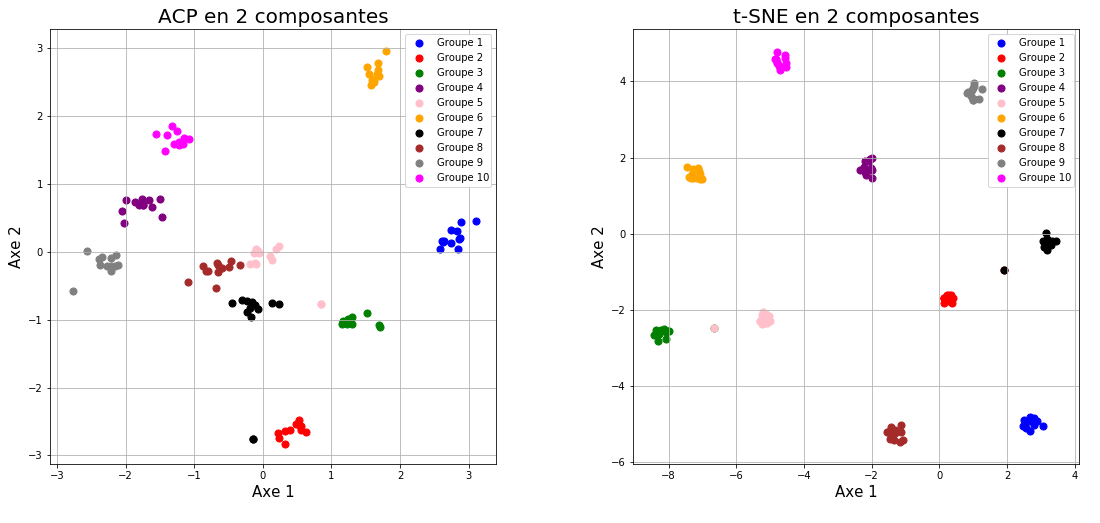
\includegraphics[width=1\textwidth]{img/figures2.png}
\captionsetup{margin=0cm,format=hang,justification=justified}
\caption{Évaluation du modèle sur données fictives.}\label{fig:figure_evaluation}
\end{center}
\vspace{-0.3cm}
\footnotesize
\emph{Note : Paramètres utilisés : ep = 50 / lr = 0,01 / w = 5 / dim = 10.}
\end{figure}

\subsection{Choix des meilleurs hyperparamètres pour le
modèle}\label{sec:hyperparametres}

Une fois nous être assurés de la bonne implémentation du modèle (partie
\ref{sec:corpusFictif}) grâce au corpus fictif, nous nous sommes
attachés à identifier les hyperparamètres les plus pertinents au regard
des données dont nous disposons.

Ces données correspondent à un ensemble de 1,3 million de
tweets\footnote{Ces tweets, fournis par Twitter, sont la propriété de
  l'Inria.} postés en France entre 2013 et 2017, supposés être
représentatifs de l'ensemble de tweets nationaux publiés durant cette
période.

Le modèle \emph{word2vec} version \emph{Skip-gram}, décrit en partie
\ref{sec:word2vec}, fait en effet intervenir un certain nombre
d'hyperparamètres parmi lesquels :

\begin{itemize}
\item $ep$ : le nombre d'\og \emph{epochs} \fg{} ;
\item $lr$ ou $\alpha$ : le \og \emph{learning rate} \fg, ou taux d'apprentissage ;
\item $w$ (\emph{window}): la taille de la fenêtre de sélection des mots contextes ;
\item $dim$ : la dimension des vecteurs-mots (ou \emph{word-embeddings}).
\end{itemize}

Or, la performance de nombreuses méthodes de \emph{machine learning},
dont \emph{word2vec}, dépend fortement des valeurs choisies pour ces
paramètres, ces valeurs étant elles-mêmes très dépendantes des données
mobilisées.

Même si les méthodes d'optimisation bayésiennes deviennent de plus en
plus performantes pour optimiser la valeur de ces hyperparamètres en
tenant compte de leurs interactions (\cite{Hutter}), ce choix s'effectue
régulièrement de manière empirique, en testant différentes valeurs
d'hyperparamètres sur les données mobilisées. C'est l'approche que nous
retenons ici.

Le package \texttt{Gensim} (\og Generate Similar \fg{}), dans lequel la
méthode \emph{word2vec} est implémentée, est un des outils actuels les
plus robustes et performants\footnote{Grâce à sa dépendance à
  \texttt{NumPy}, \texttt{Gensim} puise dans des bibliothèques de bas
  niveau. Ainsi, alors que le code de haut niveau est du Python, c'est
  en fait du Fortran et du C hautement optimisés qui sont utilisés, ce
  qui rend \texttt{Gensim} bien plus performant que \texttt{PyTorch} que
  nous avons utilisé pour implémenter le modèle décrit en partie
  \ref{sec:word2vec}.} pour la modélisation sémantique non supervisée
(\cite{Rehurek}).

Nous avons choisi de mobiliser \texttt{Gensim} dans la suite de ce
rapport, en parallèle du modèle que nous avons implémenté, en raison de
son temps d'exécution bien plus rapide\footnote{À titre d'exemple, alors
  qu'une epoch sur l'ensemble des tweets met une vingtaine d'heures à
  tourner pour \og notre \fg{} modèle, elle met 1 minute via
  \texttt{Gensim}.}. Cette rapidité d'exécution nous a permis de
réaliser des tests d'hyperparamètres plus nombreux.

Pour réaliser ces tests, nous avons fait tourner le modèle
\emph{word2vec} plusieurs fois en modifiant un à un les paramètres. Nous
avons ensuite évalué ces différents modèles par la méthode du
\og jugement humain \fg{} (partie \ref{sec:jugementHumain}) en comparant
la mesure de la similarité cosinus\footnote{Nous avons également évalué
  les modèles en utilisant (l'inverse de) la distance euclidienne à la
  place de la similarité cosinus. L'effet des paramètres devient alors
  bien moins clair et la performance du modèle est inférieure, ce va
  dans le sens de l'utilisation plus fréquente de la méthode de la
  similarité cosinus dans la littérature.} entre deux mots obtenue à
partir de notre modèle à l'évaluation subjective de cette proximité par
des individus. En outre, un même modèle est lancé six fois (six
\og seeds \fg{} différentes) afin de construire des intervalles de
confiance de la matière décrite en partie \ref{sec:jugementHumain}, en
empilant les six échantillons de mesure de proximités correspondant aux
six implémentations d'un même modèle\footnote{Pour chaque modèle, nous
  calculons les statistiques de rang des 65 paires de mots de la base de
  jugement humain ainsi que le rang des similarités cosinus des mots
  obtenus en sortie du modèle. Nous réalisons ces actions pour les six
  implémentations du même modèle et empilons les résultats obtenus.
  C'est à partir de cette base empilée de 6x65 lignes moins les données
  manquantes que nous calculons chaque intervalle de confiance selon la
  formule décrite en partie \ref{sec:jugementHumain}.}.

\subsubsection{Nombre d'epochs, taille de fenêtre et taux
d'apprentissage}\label{nombre-depochs-taille-de-fenuxeatre-et-taux-dapprentissage}

Pour cette première série de tests d'hyperparamètres, nous avons fixé la
dimension des \emph{word-embeddings} à 50 et évalué l'impact du nombre
d'epochs, de la taille de la fenêtre et du taux d'apprentissage
(figure~\ref{fig:evaluation_1}) .

\begin{figure}[htp]
\begin{center}
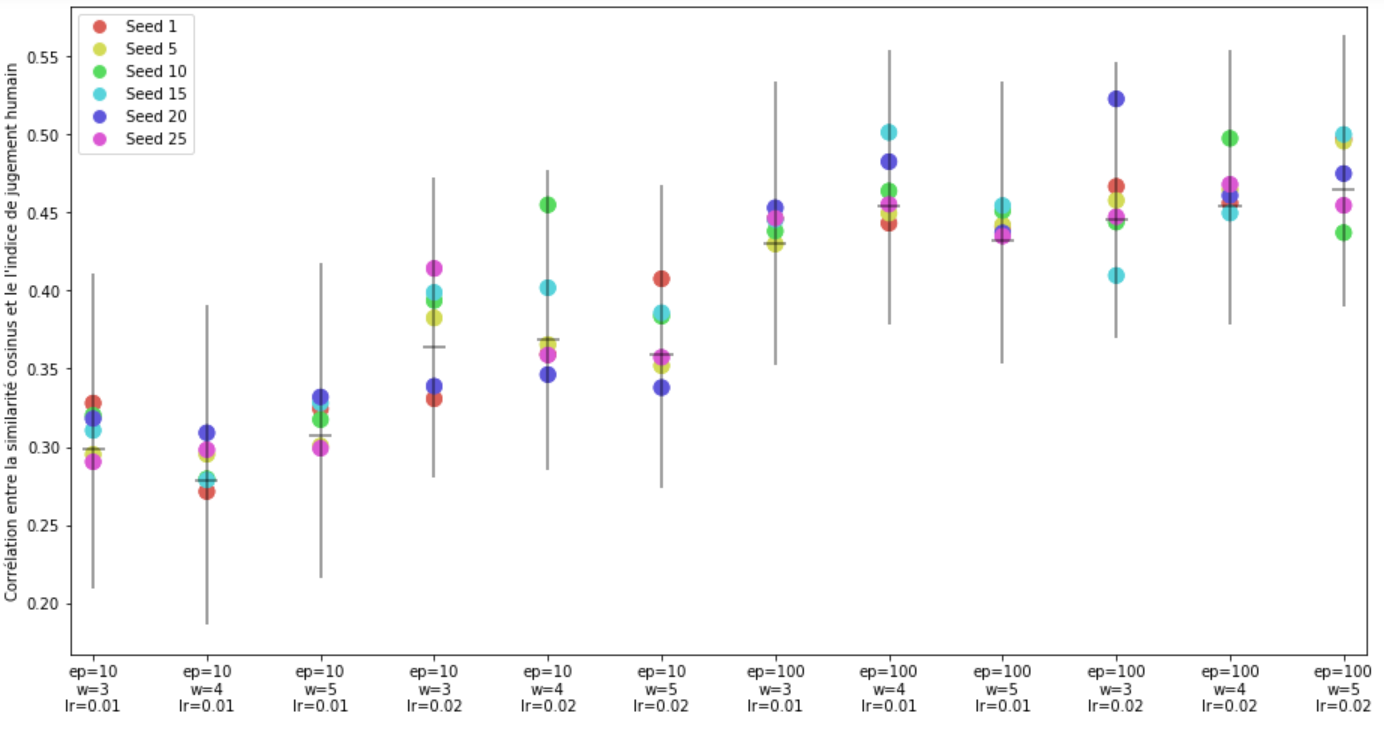
\includegraphics[width=1\textwidth]{img/test_parametres.png}
\captionsetup{margin=0cm,format=hang,justification=justified}
\caption{Tests d'hyperparamètres : epochs, fenêtre et taux d'apprentissage.}\label{fig:evaluation_1}
\end{center}
\vspace{-0.3cm}
\footnotesize
\emph{Note : Paramètre utilisé : dim = 50\newline
Le trait horizontal correspond au coefficient de Spearman calculé sur les échantillons empilés des six modèles et la barre verticale à l'intervalle de confiance associé.}
\end{figure}

\paragraph{Le nombre d'epochs}\label{le-nombre-depochs}

~

Le nombre d'epochs a un effet net. Passer de 10 à 100 epochs fait
nettement augmenter le score de corrélation de Spearman entre données
subjectives et données en sortie du modèle.

\faArrowCircleRight{} Nous retenons alors le paramètre \textbf{ep =
100}.

\paragraph{Le taux d'apprentissage}\label{le-taux-dapprentissage}

~

La valeur 0,02 semble donner systématiquement de meilleurs résultats que
0,01.

En réalisant davantage de tests de taux d'apprentissage en fixant les
autres hyperparamètres, les différents taux d'apprentissage présentent
des performances similaires\footnote{En fixant les paramètres dim = 50,
  ep = 100 et w = 4 (celles du modèle retenu \emph{in fine}), et en
  testant les taux d'apprentissage 0,005, 0,01, 0,02, 0,03 et 0,04, les
  valeurs moyennes des corrélations s'échelonnent entre 0,41 et 0,48,
  soit des valeurs proches.}.

\faArrowCircleRight{} Nous retenons alors le paramètre \textbf{lr =
0,02}.

\paragraph{La taille de la fenêtre}\label{la-taille-de-la-fenuxeatre}

~

La taille de la fenêtre ne semble pas jouer un rôle majeur, et dépend
beaucoup des autres paramètres choisis.

Certains travaux (\cite{Levy2}) indiquent que, suivant la taille de
fenêtre choisie, les informations capturées sont différentes. Cela
pourrait expliquer la complexité de choisir la \og meilleure \fg taille
de fenêtre. Alors que les \og grandes \fg fenêtres capturent des
informations sur le domaine du mot (autres mots de tout type étant
utilisés dans des discussions connexes), les \og petites \fg fenêtres
saisissent davantage le mot en lui-même (ses extensions, synonymes, lui
sont alors proches). La valeur de 4 représente une taille de fenêtre
\og ni trop grande ni trop petite\fg et qui présente de bons résultats
dans la plupart des tests effectués.

\faArrowCircleRight{} Nous retenons alors le paramètre \textbf{w = 4}.

\subsubsection{Dimension des
vecteurs-mots}\label{dimension-des-vecteurs-mots}

On cherche cette fois-ci à évaluer l'effet de la dimension des
\emph{word-embeddings}. Selon certains papiers (comme
\cite{Pennington}), la qualité des représentations vectorielles
s'améliore à mesure que l'on augmente la taille du vecteur, mais
seulement jusqu'à atteindre 300 dimensions\footnote{La dimension des
  vecteurs doit également être adaptée à la taille du vocabulaire.
  \cite{Mikolov} recommande donc d'augmenter à la fois la dimension des
  vecteurs et la quantité de données d'apprentissage. Par exemple, avec
  un vocabulaire d'une centaine de mots, il serait inefficace d'utiliser
  des projections en grande dimension (risque de surapprentissage).}.
Après 300 dimensions, la qualité des vecteurs commence à diminuer et le
temps de calcul augmente considérablement.

\begin{figure}[htp]
\begin{center}
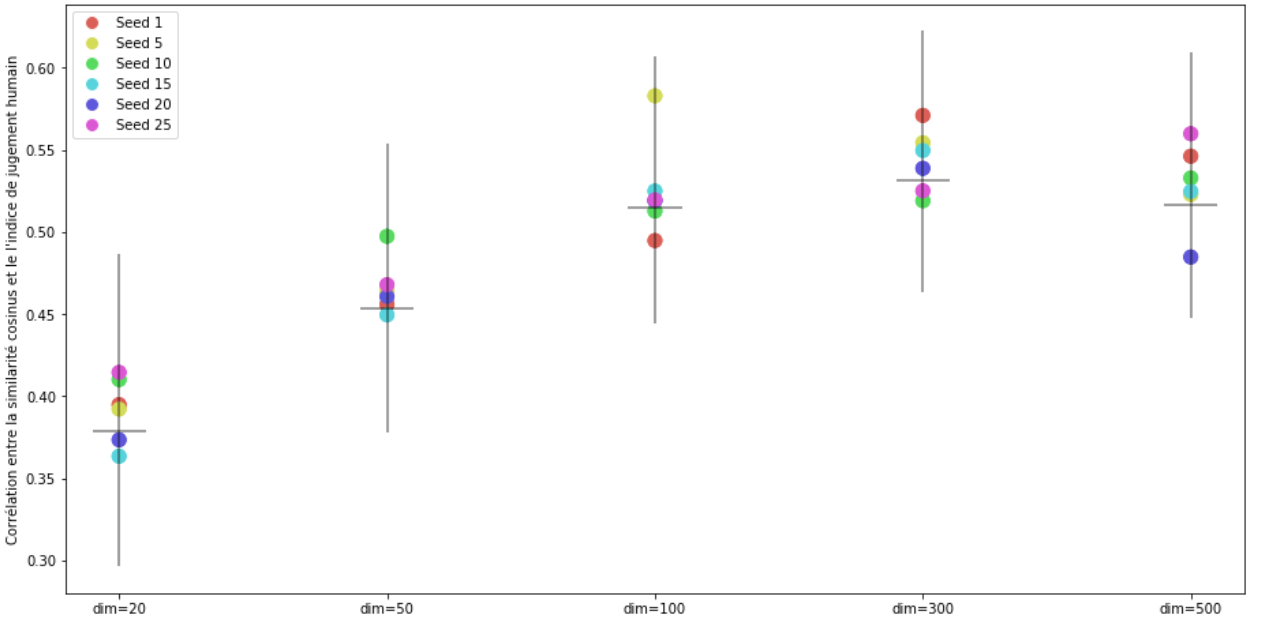
\includegraphics[width=1\textwidth]{img/test_parametres2.png}
\captionsetup{margin=0cm,format=hang,justification=justified}
\caption{Tests d'hyperparamètres : dimension des \emph{word-embeddings}.}\label{fig:figure_dim}
\end{center}
\vspace{-0.3cm}
\footnotesize
\emph{Note : Paramètres utilisés : ep = 100 / w = 4 / lr = 0,02.\newline
Le trait horizontal correspond au coefficient de Spearman calculé sur les échantillons empilés des six modèles et la barre verticale à l'intervalle de confiance associé.}
\end{figure}

En pratique, en comparant l'effet de la dimension des vecteurs (modèle
fixé à ep~=~100, w~=~4 et lr~=~0,02), on observe bien une augmentation
de l'efficacité du modèle jusqu'en dimension 300 et une efficacité
moindre en dimension 500 (figure~\ref{fig:figure_dim}). Bien que
l'efficacité du modèle semble meilleure en dimension 300, la dimension
100 améliore la rapidité de l'algorithme, pour des résultats d'une
qualité similaire.

\faArrowCircleRight{} Nous retenons alors le paramètre \textbf{dim =
100}.

\subsection{Évaluation sur le corpus
final}\label{uxe9valuation-sur-le-corpus-final}

\subsubsection{\texorpdfstring{Avec \og notre
\fg modèle}{Avec notre modèle}}\label{avec-notre-moduxe8le}

Nous avons ensuite fait tourner le modèle que nous avons implémenté en
utilisant les paramètres retenus précédemment (w~=~4, lr~=~0,02 et
dim~=~100) mais uniquement sur 100~000 tweets et 80 epochs pour des
questions de temps de calcul\footnote{Pour ces paramètres, le temps de
  calcul était d'environ 18 heures.}. Les résultats obtenus semblent
relativement satisfaisants. La recherche des plus proches voisins par
similarité cosinus (dont quelques exemples sont illustrés en tableau
\ref{table:knn_ark}) donne des résultats proches de l'intuition.

\begin{table}[!h]
\begin{center}
\begin{tabular}{|c|c|c|c|}
    \hline
\textbf{bonjour} & \textbf{femme} & \textbf{1} & \textbf{samedi} \tabularnewline
\emph{(669 apparitions)} & \emph{(264 apparitions)} & \emph{(765 apparitions)} & \emph{(203 apparitions)} \tabularnewline
       \hline

\includegraphics[height=4mm]{img/emojis/1.png} (0,59) & quelle (0,49) & 5 (0,55) & soir (0,57) \tabularnewline

\includegraphics[height=4mm]{img/emojis/2.png} (0,59) & cette (0,46) & mois (0,51) & vivement (0,51) \tabularnewline
merci (0,54) & une (0,44) & 10 (0,49) & demain (0,50) \tabularnewline
nuit (0,48) & vie (0,44) & 2 (0,48) & end (0,48) \tabularnewline
bisous (0,47) & grippe (0,44) & top (0,48) & weekend (0,47) \tabularnewline
bonne (0,47) & belle (0,43) & depuis (0,47) & matin (0,45) \tabularnewline

\includegraphics[height=4mm]{img/emojis/3.png} (0,46) & ma (0,43) & saison (0,46) & jeudi (0,45) \tabularnewline
vous (0,46) & magnifique (0,43) & ans (0,44) & prochain (0,43) \tabularnewline
plaisir (0,44) & nouvelle (0,43) & jours (0,43) & week (0,43) \tabularnewline
allez (0,43) & vidéo (0,39) & 3 (0,43) & 
\includegraphics[height=4mm]{img/emojis/4.png} (0,42) \tabularnewline
    \hline
 \end{tabular}
\captionsetup{margin=0cm,format=hang,justification=justified}
\caption{10 plus proches voisins par similarité cosinus avec \og notre \fg{} modèle.}\label{table:knn_ark}
\end{center}
\vspace{-0.3cm}
\footnotesize
\emph{Note : Paramètres utilisés : ep = 80 / w = 4 / lr = 0,02 / dim = 100 / base : 100 000 tweets\newline
La similarité cosinus de chaque paire de mots est renseignée entre parenthèses.}

\end{table}

Par ailleurs, le coefficient de Spearman entre la similarité cosinus des
mots obtenus et le jugement humain est de 0,571 (p-valeur : 4,1 \%).
Toutefois, ce bon résultat est à considérer avec précaution puisque
seuls 13 des couples de mots de la base RG-65 ont été reconnus dans le
corpus de 100~000 tweets que nous utilisons ici.

Enfin, les représentations graphiques des positions des mots via des ACP
et les sommes vectorielles sur les mots\footnote{Comme l'exemple de
  \(\overrightarrow{Paris} - \overrightarrow{France} + \overrightarrow{Italie} = \overrightarrow{Rome}\)
  dans \cite{Mikolov}} donnent des résultats bien moins concluants que
le modèle \texttt{Gensim} entraîné sur l'ensemble des tweets (partie
\ref{sec:gensimresultats}).

\subsubsection{\texorpdfstring{Avec le modèle
\texttt{Gensim}}{Avec le modèle Gensim}}\label{sec:gensimresultats}

Le modèle \texttt{Gensim} (entraîné avec les paramètres w~=~4,
lr~=~0,02, dim~=~100 et ep~=~100) donne des résultats encore plus
convaincants que précédemment, ayant été davantage entraîné, et sur un
corpus plus fourni (ensemble des tweets). En effet, les vecteurs-mots en
sortie du modèle \texttt{Gensim} sur l'ensemble des tweets (figure
\ref{fig:acp_freq_gensim}) sont davantage répartis dans l'ensemble du
plan, alors que les mots en sortie du modèle que nous avons implémenté
sur 100 000 tweets sont répartis en fonction de leur nombre
d'occurrences, les mots les moins fréquents n'ayant probablement pas (ou
peu) été entraînés (figure \ref{fig:acp_freq_ark}).

\begin{figure}[h]
\begin{minipage}{.5\textwidth}
  \centering
  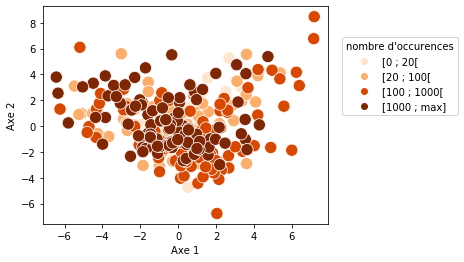
\includegraphics[width=1\linewidth]{img/acp_freq_gensim.png}
  \captionof{figure}{Position des mots en fonction de\newline leur nombre d'occurrences (modèle \texttt{Gensim}).}
  \label{fig:acp_freq_gensim}
\end{minipage}%
\begin{minipage}{.5\textwidth}
  \centering
  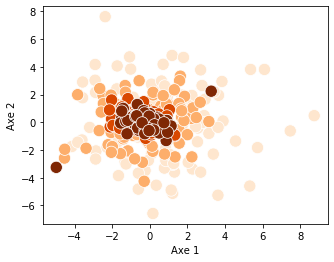
\includegraphics[width=0.72\linewidth]{img/acp_freq_ark.png}
  \captionof{figure}{Position des mots en fonction de\newline leur nombre d'occurrences (\og notre \fg{} modèle).}
  \label{fig:acp_freq_ark}
\end{minipage}
\footnotesize
\emph{Note : Paramètres utilisés : ep = 100 (gauche) ou 80 (droite) / w = 4 / lr = 0,02 / dim = 100.\newline
Méthode utilisée : ACP, deux premiers axes.}
\end{figure}

Le coefficient de Spearman a une valeur semblable à précédemment : 0,495
mais sa p-valeur est proche de 0 \% et, cette fois-ci, 52 des couples de
mots de la base RG-65 ont été reconnus dans le corpus de tweets.

Les 10 plus proches voisins calculés par similarité cosinus (tableau
\ref{table:knn_gensim}) semblent encore plus pertinents. Les plus
proches voisins de \og \(1\) \fg contiennent davantage de chiffres, ceux
de \og samedi \fg davantage de jours de la semaine et le tableau
contient désormais des synonymes de \og femme \fg et de \og bonjour \fg.
Certains mots surprenants subsistent toutefois, comme par exemple
\og transmets \fg{}, \og désagrément \fg{} et \og betembourg \fg{},
voisins de \og bonjour \fg{}. Toutefois, la fréquence d'apparition de
ces mots dans le corpus est faible (moins d'une centaine d'occurrences).
La projection de certains vecteurs-mots sur les deux premiers axes d'une
ACP (figure \ref{fig:acp_gensim}) nous confirme la qualité de
l'entraînement du corpus sur l'ensemble de tweets.

\begin{table}[h]
\begin{center}
\begin{tabular}{|c|c|c|c|}
    \hline
\textbf{bonjour} & \textbf{femme} & \textbf{1} & \textbf{samedi} \tabularnewline
\emph{(17 043 apparitions)} & \emph{(6 177 apparitions)} & \emph{(21 055 apparitions)} & \emph{(4 917 apparitions)} \tabularnewline
       \hline
bonsoir (0,85) & fille (0,86) & 2 (0,65) & vendredi (0,88) \tabularnewline
bjr (0,75) & copine (0,74) & 3 (0,64) & jeudi (0,86) \tabularnewline
hello (0,71) & meuf (0,71) & 6 (0,63) & lundi (0,83) \tabularnewline
salut (0,66) & demoiselle (0,66) & 4 (0,62) & mercredi (0,83) \tabularnewline
coucou (0,55) & nana (0,66) & 7 (0,60) & dimanche (0,83) \tabularnewline
transmets (0,49) & nièce (0,66) & 5 (0,58) & mardi (0,76) \tabularnewline
désagrément (0,48) & sœur (0,65) & 9 (0,58) & demain (0,72) \tabularnewline
avezvous (0,48) & barbe (0,65) & 8 (0,56) & barathon (0,56) \tabularnewline
bettembourg (0,48) & maman (0,64) & 1e (0,55) & 22h45 (0,55) \tabularnewline
hey (0,47) & princesse (0,64) & 34 (0,53) & 20h (0,54) \tabularnewline
    \hline
 \end{tabular}
\captionsetup{margin=0cm,format=hang,justification=justified}
\caption{10 plus proches voisins par similarité cosinus avec le modèle \texttt{Gensim}.}\label{table:knn_gensim}
\end{center}
\vspace{-0.3cm}
\footnotesize
\emph{Note : Paramètres utilisés : ep = 100 / w = 4 / lr = 0,02 / dim = 100 / base : ensemble des tweets\newline
La similarité cosinus de chaque paire de mots est renseignée entre les parenthèses.}
\end{table}

\begin{figure}[!h]
\begin{center}
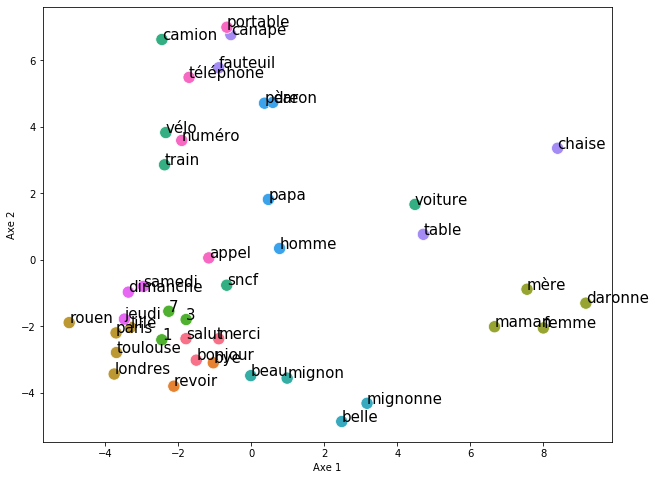
\includegraphics[width=0.5\textwidth]{img/acp_gensim.png}
\captionsetup{margin=0cm,format=hang,justification=justified}
\caption{ACP sur un corpus réduit de mots.}\label{fig:acp_gensim}
\end{center}
\vspace{-0.3cm}
\footnotesize
\emph{Note : Paramètres utilisés : ep = 100 / w = 4 / lr = 0,02 / dim = 100 / base : ensemble des tweets }
\end{figure}

\begin{figure}[!h]
\begin{minipage}{.5\textwidth}
  \centering
  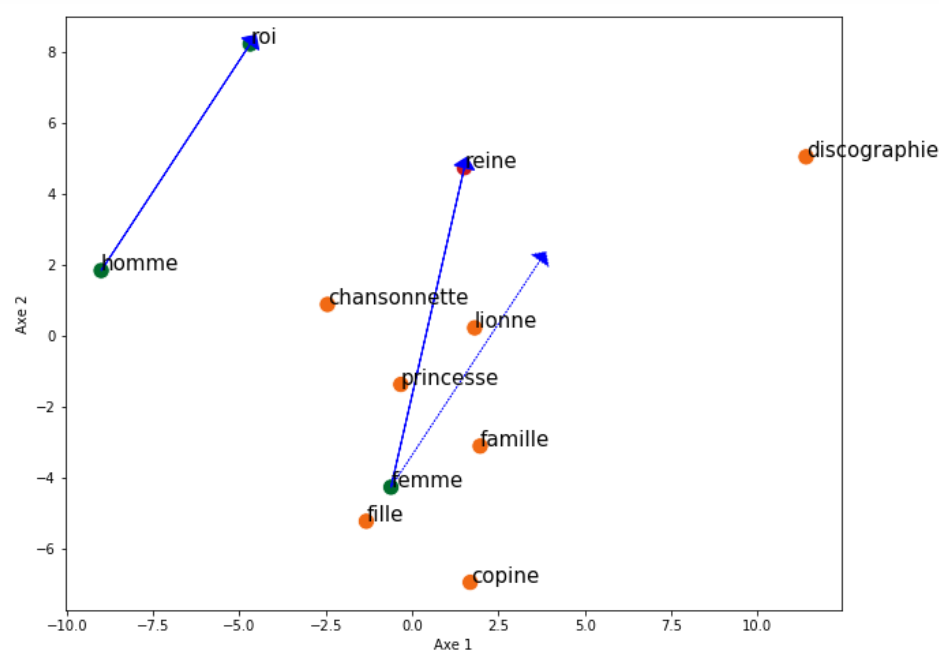
\includegraphics[width=0.92\linewidth]{img/acp_reine.png}
  \captionof{figure}{\ $\protect\overrightarrow{Roi} - \protect\overrightarrow{Homme} + \protect\overrightarrow{Femme} = $ ?}
  \label{fig:acp_reine}
\end{minipage}%
\begin{minipage}{.5\textwidth}
  \centering
  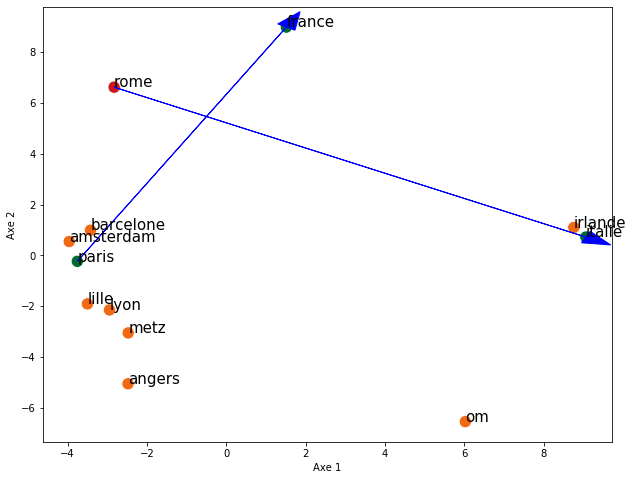
\includegraphics[width=0.85\linewidth]{img/acp_rome.png}
  \captionof{figure}{\ $\protect\overrightarrow{Paris} - \protect\overrightarrow{France} + \protect\overrightarrow{Italie} = $ ?}
  \label{fig:acp_rome}
\end{minipage}
\footnotesize
\emph{Note : Paramètres utilisés : ep = 100 / w = 4 / lr = 0,02 / dim = 100.\newline
Les mots en vert correspondent à ceux à gauche de l'opération, le mot en rouge à celui que l'on serait supposé trouver et les mots en orange les 10 mots les plus proches du résultat de l'opération vectorielle.}
\end{figure}

Enfin, nous avons réalisé des opérations sur les mots-vecteurs. Si
l'opération
\(\overrightarrow{Roi} - \overrightarrow{Homme} + \overrightarrow{Femme} = \overrightarrow{Reine}\)
(figure \ref{fig:acp_reine}) semble fonctionner \footnote{Les
  similarités cosinus obtenues sont les suivantes :
  \(corr(\overrightarrow{Roi}, \overrightarrow{Homme}) = 0,34\),
  \(corr(\overrightarrow{Homme}, \overrightarrow{Femme}) = 0,35\) et
  \(corr(\overrightarrow{Roi} - \overrightarrow{Homme} + \overrightarrow{Femme} , \overrightarrow{Reine}) = 0,67\).
  \(\overrightarrow{Reine}\) est bien le mot le plus proche de la somme
  vectorielle calculée.}, l'opération
\(\overrightarrow{Paris} - \overrightarrow{France} + \overrightarrow{Italie}\)
(figure \ref{fig:acp_rome}) n'identifie pas \og Rome \fg{} (similarité
cosinus de 0,18 seulement) dans les mots les plus proches mais d'autres
villes comme \og Lyon \fg{} (similarité cosinus de 0,62). \og Rome \fg{}
semble effectivement située \og trop en haut\fg{} dans le plan de l'ACP
par rapport aux autres villes. Peut-être ce mot n'a-t-il pas
suffisamment été entraîné (246 apparitions dans les tweets contre 46 433
pour Lyon par exemple) pour que le vecteur-mot obtenu soit pertinent, ou
peut-être que, dans les tweets mobilisés, le mot \og Rome \fg{}
s'utilise dans un contexte différent que le corpus utilisé dans
\cite{Mikolov}.

\section{Construction d'un indice mensuel de sentiment moyen des
tweets}\label{sec:sentimentalAnalysis}

Afin de créer un indice mensuel de sentiment moyen des tweets, nous
allons utiliser les vecteurs-mots obtenus en sortie du modèle
\emph{word2vec} couplés avec une base de tweets annotée en termes de
sentiment. Cette base contient un ensemble de tweets sur les transports
urbains tous qualifiés de positifs ou négatifs. Nous comparerons ensuite
cet indicateur avec l'indicateur synthétique de confiance des ménages
(Camme, Insee). L'ensemble de ces données sont décrites dans l'encadré
\ref{enc:encadre1}.

\begin{encadre}[true]{Données utilisées}\label{enc:encadre1}

\small

\textbf{Tweets mensuels}

Il s'agit de la base des tweets postés en France utilisée précédemment (partie  \ref{sec:hyperparametres}) mais couvrant un horizon temporel plus large (2011-2018).
Nous disposons de 4 200 tweets pour tous les mois de la période sous-échantillonnés de manière à avoir autant de tweets pour certains jours (les 1, 5, 10, 15, 20, 25 et 28 de chaque mois) et heures (0h, 6h, 12h 15h 18h et 21h) fixés. 

\textbf{Tweets annotés sur les transports urbains}

Cette base est composée d'environ 23 000 tweets qui concernent les transports urbains (trains SNCF, métros et bus de la RATP) annotés en termes de sentiment.
Nous avons transformé cette annotation de manière à associer une valeur de $+1$ à un tweet considéré comme positif et de $0$ à un tweet considéré comme négatif.


\textbf{Indicateur synthétique de confiance des ménages}

L’indicateur synthétique de confiance des ménages provient de l'Enquête mensuelle de conjoncture auprès des ménages (Camme) de l’Insee.
Il décrit, en une variable unique, la composante commune de 8 soldes d’opinion qui correspondent à la différence entre les pourcentages de réponses positives et négatives sur différents sujets (niveau de vie passé et futur en France, situation financière personnelle passée et future, perspective de chômage, opportunité de faire des achats importants, capacité à épargner actuelle et dans les mois à venir). Les réponses \og ne sait pas \fg n'entrent donc pas dans le calcul des soldes d'opinion.
L'indicateur synthétique est calculé par analyse factorielle statique, dont l’objectif est de résumer l’évolution concomitante de ces soldes aux évolutions très corrélées.
Il s’interprète surtout en évolution et il est normalisé de manière à avoir une moyenne de 100 et un écart-type de 10. 

\end{encadre}

\subsection{Prédire le sentiment d'un
tweet}\label{pruxe9dire-le-sentiment-dun-tweet}

Nous cherchons dans cette partie à construire un modèle permettant de
prédire le sentiment (\(0\) pour négatif ou \(1\) pour positif) associé
à un tweet à partir des mots qui le composent. Nous utilisons pour cela
la base annotée sur les transports (encadré \ref{enc:encadre1}). Nous
comparerons deux approches : une première basée sur le lexique
(\emph{lexicon-based}) et plus précisément sur les sentiments moyens de
chaque mot des tweets (partie \ref{sec:sentiments}) qui servira de
référence pour évaluer l'efficacité de la seconde approche basée sur une
régression binaire sur les \emph{word-embeddings} (partie
\ref{sec:wordembeddings}).

\subsubsection{Modèle lexical : prédiction à partir du sentiment moyen
des mots}\label{sec:sentiments}

Ce premier modèle lexical (\emph{lexicon-based}) de prédiction du
sentiment utilise l'information des tweets labelisés pour déterminer un
sentiment moyen par mot. Le sentiment prédit d'un tweet \(t\) composé de
\(n\) mots sera :
\[S_{1,\gamma}(t) = \mathds{1}\left\{ \frac{1}{n} \sum \limits_{i=1}^n \alpha_i \geq \gamma\right\}  \qquad \in \{ 0,1 \}\]
avec \(\gamma \in [-1,1]\) un seuil fixé,
\(\alpha_i = \frac{nb_+(i) - nb_-(i)}{nb_+(i) + nb_-(i)} \in [-1,1]\) le
sentiment moyen du mot \(i\) calculé à partir du nombre de tweets
positifs (\(nb_+(i)\)) et négatifs (\(nb_-(i)\)) dans lesquels il
apparaît.

Afin d'évaluer l'efficacité du modèle, nous séparons la base de tweets
annotés sur les transports en une base d'entraînement (environ 16 000
tweets) et une base de test (environ 7 000 tweets)\footnote{13 \% des
  mots du vocabulaires et 1 \% des mots utilisés dans les tweets de la
  base test sont absents de la base d'entraînement. Pour ces mots, le
  sentiment moyen \(\alpha_i\) est fixé à 0.}. La base d'entraînement
sert à calculer les sentiments moyens des mots et à déterminer le
\(\gamma\) qui présente les meilleures performances, et la base de test
permet d'estimer le modèle, c'est-à-dire prédire pour chaque tweet un
sentiment, que l'on compare au vrai sentiment.

On choisit \(\gamma\) tel que l'\emph{accuracy} sur la base
d'entraînement\footnote{Dans notre base d'entraînement, la proportion de
  tweets positifs (43 \%) est proche de la proportion de tweets négatifs
  (57 \%). Il n'y a donc pas de problème de déséquilibre des classes :
  maximiser l'\emph{accuracy} permet bien de maximiser la performance de
  l'algorithme.} --- c'est-à-dire le taux de tweets dont le sentiment
est bien prédit --- soit maximale. On obtient \(\gamma^* = -0,14\)
(figure \ref{fig:max_baseline}). En évaluant le modèle sur la base de
test, l'\emph{accuracy} vaut 89,1 \%. On constate une nette amélioration
par rapport au cas où \(\gamma = 0\) (70,5 \%), qui correspond au seuil
«~naturel~» puisqu'il se situe au centre de l'intervalle des valeurs
possibles pour \(\alpha_i\).

\begin{figure}[h]
\begin{center}
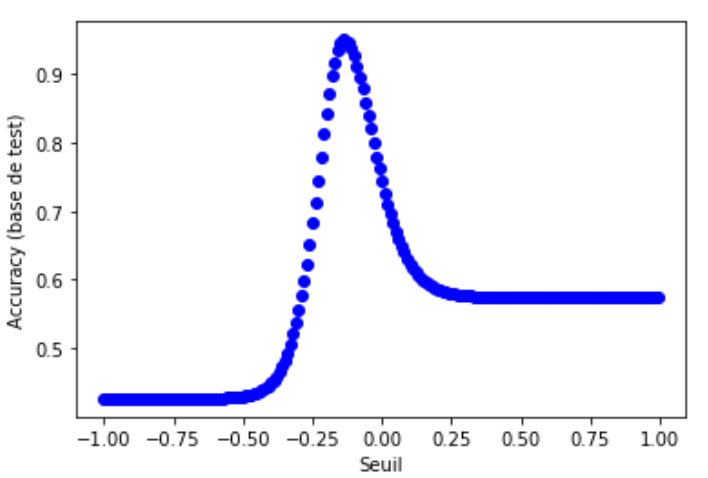
\includegraphics[width=0.5\textwidth]{img/max_baseline.png}
\captionsetup{margin=0cm,format=hang,justification=justified}
\caption{Optimisation du seuil $\gamma$ pour le modèle lexical.}\label{fig:max_baseline}
\end{center}
\end{figure}

\subsubsection{\texorpdfstring{Modèle logit : prédiction à partir des
\emph{word-embeddings}}{Modèle logit : prédiction à partir des word-embeddings}}\label{sec:wordembeddings}

Nous nous intéressons maintenant à un modèle basé sur l'utilisation de
nos \emph{word-embeddings}. Pour cela, nous utilisons un modèle de
régression binaire avec comme prédicteurs chacune des 100 dimensions des
vecteurs-mots. Toutefois, comme il s'agit ici de prévoir le sentiment
des tweets et non de mots, une première étape préalable est de
transformer pour chaque tweet l'ensemble des \emph{word-embeddings} des
mots qui le composent en une «~\emph{sentence-embedding}~» qui
correspondra à la moyenne des vecteurs-mots.

Le modèle prédictif binaire est de la forme : \[
Y_i = \mathds{1}\left\{ \sum_{i = 1}^n \beta_i X_{i,j} + \varepsilon_i \geq 0 \right\} 
\quad 
\text{et nous prédisons} 
\quad  
\mathbb{P}(Y_i = 1 | X_{i}) = F_{\varepsilon}\left(\sum_{i = 1}^n \beta_i X_{i,j}\right)
\] Avec :

\begin{itemize}
\item $Y_i$ le sentiment du tweet $i$ ;
\item $X_{i,1}, \dots, X_{i,n}$ les coordonnées de la \emph{sentence-embedding} du tweet $i$ ;
\item $\varepsilon_i$ le résidu de notre modèle, de fonction de répartition $F_{\varepsilon}$ qui vaudra $F_{\varepsilon}(x) = \frac{1}{1 + e^{-x}}$ dans le cas d'un modèle logit et $F_{\varepsilon}(x) = \Phi(x)$ (fonction de répartition d'une loi $\mathcal{N}(0, 1)$) dans le cas d'un modèle probit. 
\end{itemize}

Puis nous appliquons le critère de classification suivant pour prédire
le sentiment \(S_{2,\gamma}(t) \in \{0,1\}\) du tweet \(t\) avec le
seuil \(\gamma = 0,5\) :

\[S_{2,\gamma}(t) = \mathds{1}\left\{   \mathbb{P}(Y_i = 1 | X_{i}) \ge \gamma\right\} \qquad \in \{0,1\}\]

Afin de sélectionner le meilleur modèle, nous avons comparé 8 modèles
comportant différentes spécifications en utilisant le critère de l'AUC
(aire sous la courbe ROC\footnote{La courbe ROC permet de représenter
  pour l'ensemble des seuils possibles l'évolution du nombre de vrais
  positifs en fonction du nombre de faux positifs. L'AUC, l'aire sous
  cette courbe, est donc compris entre 0 et 1. Une valeur proche de 0,5
  correspond à un modèle aléatoire. À l'inverse, une AUC proche de 1
  correspond à un très bon modèle prédictif.}) par validation
croisée\footnote{Nous avons réalisé une \emph{k-fold cross validation}
  qui est une technique permettant de limiter le surapprentissage sur la
  base de test. Le principe est de découper la base en \(k = 10\)
  échantillons puis de considérer tour à tour chaque échantillon comme
  base de test, en entraînant le modèle sur les \(k-1\) échantillons
  restants. On calcule alors l'AUC dans chaque cas, puis on en calcule
  la moyenne.}. Les différences spécifications testées sont les
suivantes :

\begin{enumerate}
\item \textbf{L’inclusion ou non des \emph{stop words}} (mots-vides). 
Ces mots sont des mots communs qui, en général, n’apportent pas d’information cruciale dans l’analyse textuelle. 
Les comparaisons de modèles indiquent qu’enlever ces mots n’améliore pas les performances de prédiction et les détériore même légèrement. 
Cela peut s’expliquer par le fait que certains mots-vides renseignent sur un sentiment comme par exemple le mot « pas » qui pourrait contribuer à qualifier des tweets de négatifs (son sentiment moyen dans le corpus est de $-0,25$).

\item \textbf{Le traitement des mots inconnus}. 
La base qui a servi à constituer les \emph{word-embeddings} avec \emph{word2vec} est différente de celle que l'on utilise pour la prédiction des sentiments.
Ainsi, il existe des mots dont on ne connaît pas la représentation vectorielle. 
Deux options ont été retenues pour traiter ces mots. 
La première est de les retirer des tweets analysés afin qu'ils n’influent pas sur la décision du sentiment. 
La seconde est de leur attribuer la valeur du vecteur correspondant aux mots rares (vecteur « lowfrequency », voir partie \ref{subsec:baseentrainement}) en partant du principe que s'ils sont absents du corpus d'entraînement du modèle \emph{word2vec}, ce sont bien des mots très peu fréquents. 
C’est cette deuxième option qui semble donner des résultats légèrement meilleurs, ce qui peut signifier que l’on capte alors le fait que les mots peu fréquents ne sont en moyenne pas neutres (plutôt positifs ou négatifs\footnote{En utilisant le modèle logit retenu, la prévision d'une \emph{sentence-embedding} composée uniquement du mot « lowfrequency » donne $\widehat{\mathbb{P}}(Y_i = 1 | X_{lowfrequency}) = 0,87$, ce qui laisse supposer que les mots-rares ont une consonance davantage positive.}). 

\item \textbf{La modélisation probit ou logit}. En plus de comparer les AUC des différentes spécifications ci-dessus, on compare à spécification fixée les modèles logit et probit avec des critères économétriques (AIC, BIC). C’est le modèle logit qui permet d’obtenir les meilleurs résultats, quels que soient les choix faits par ailleurs concernant les mot-vides et les mots inconnus.

\end{enumerate}

Finalement, nous retenons le modèle estimé par une \textbf{régression
logit} sur la base en \textbf{gardant les mots-vides} et en affectant
aux mots inconnus le \textbf{vecteur des mots très peu fréquents}.
L'\emph{accuracy} de ce modèle est de 69,8 \%\footnote{Cette valeur de
  l'\emph{accuracy} correspond au seuil \(\gamma = 0,5\). Comme dans la
  partie précédente, nous avons déterminé le seuil optimal sur la base
  de d'entraînement et comme celui-ci était très proche de 0,5
  (\(\gamma^* = 0,49\)), pour une \emph{accuracy} de seulement 70,0 \%,
  nous avons conservé le seuil médian de \(0,5\).}, valeur inférieure au
modèle lexical (89,1 \%).

\subsubsection{Les limites des modèles
utilisés}\label{les-limites-des-moduxe8les-utilisuxe9s}

La bonne performance du modèle lexical (sentiment moyen des mots par
tweet) par rapport au modèle logit (sur les \emph{sentence-embeddings})
peut s'expliquer par plusieurs facteurs.

\paragraph{Les mots inconnus}\label{les-mots-inconnus}

Une première explication est la différence entre les deux modèles en
termes de mots inconnus. Nous l'avons vu, pour le modèle lexical, 1,4 \%
des mots utilisés dans les tweets de la base test des tweets sur les
transports (13,2 \% du vocabulaire) sont absents de la base
d'entraînement. Pour le modèle logit basé sur les
\emph{sentence-embeddings}, il faut mécaniquement ajouter aux mots
inconnus ceux pour lesquels nous ne disposons pas de vecteurs-mots.
Ainsi, les mots inconnus sont bien plus nombreux puisqu'ils représentent
4,6 \% des mots (36,2 \% du vocabulaire).

Toutefois, la présence de mots inconnus ne semble pas biaiser la
prédiction du sentiment d'un tweet. En effet, la distribution de la part
des mots inconnus est étonnamment similaire quand on se restreint aux
tweets bien prédits et à ceux mal prédits (figure
\ref{fig:mots_inconnus}).

\begin{figure}[ht]
\begin{center}
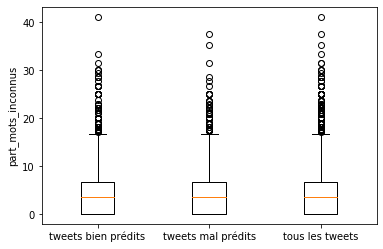
\includegraphics[width=0.5\textwidth]{img/mots_inconnus.png}
\captionsetup{margin=0cm,format=hang,justification=justified}
\caption{Part des mots inconnus dans les tweets.}\label{fig:mots_inconnus}
\end{center}
\end{figure}

\paragraph{Le processus d'annotation utilisé pour les tweets sur les
transports
urbains}\label{le-processus-dannotation-utilisuxe9-pour-les-tweets-sur-les-transports-urbains}

L'éventualité que le modèle lexical reproduise en partie le processus
qui a été utilisé pour générer les sentiments de la base sur les
transports urbains pourrait également être une explication de la
surperformance du modèle lexical. En effet, nous ne disposons pas de la
méthodologie qui a permis d'annoter ces tweets et nous avons pu relever
quelques incohérences dans les sentiments attribués à certains tweets.
Cela peut laisser supposer que l'annotation n'a pas été purement
manuelle. Comme de nombreux autres, le tweet ci-dessous, très
vraisemblablement ironique, a par exemple été qualifié de positif.

\begin{quote}
\LARGE \textbf{``}\normalsize \emph{C'est cool de payer un abonnement de 180 euros par mois pour attendre 1h le bus.} \LARGE \textbf{''}\normalsize
\end{quote}

\paragraph{\texorpdfstring{Le
\emph{domain-shift}}{Le domain-shift}}\label{le-domain-shift}

Une dernière explication possible pourrait être ce qu'on appelle le
\emph{« domain shift »} ou changement de domaine. Les techniques
d'apprentissage automatique sont souvent confrontées à un défi majeur :
le fait que les modèles soient entraînés sur des données différentes de
celles que l'on va effectivement utiliser, c'est ce que l'on appelle le
\emph{dataset shift}\footnote{Les éléments en lien avec le \emph{dataset shift}, et plus particulièrement le \emph{domain shift}, proviennent de \cite{Candela}}.
Bien que des solutions comme la correction de biais de sélection des
échantillons, ou encore celle des données déséquilibrées, soient
étudiées depuis de nombreuses décennies dans le monde de la statistique,
certains autres problèmes, comme celui du changement de domaine
(\emph{domain shift}) émergent depuis plus récemment suite à
l'utilisation croissante des méthodes de \emph{machine learning}.

Le changement de domaine se caractérise par un changement de la nature,
du «~domaine~» des données utilisées. Dans le cas de
\emph{deep-learning} sur des données de photographie, il pourrait par
exemple s'agir de traiter de corpus de photos prises par des appareils
photo calibrés de manières différentes (contraste, luminosité\dots) .
Dans notre cas précis, il s'agit de la différence entre les données de
tweets publiés en France entre 2013 et 2017 et les données de tweets sur
les transports urbains. Ces derniers portent sur un sujet très
spécifique et certains mots ont peut-être une interprétation spécifique
en termes de sentiments. Modéliser le \emph{domain shift} implique donc
d'estimer le passage d'une représentation à une autre en utilisant des
informations de distribution\footnote{La correction gamma
  (représentation paramétrique non linéaire de l'intensité des pixels)
  est par exemple une manière de pouvoir traiter le \emph{domain shift}
  lié à l'utilisation d'appareils photo différents.}.

L'idée n'est pas ici de modéliser mathématiquement le \emph{domain
shift}\footnote{En quelques mots, pour modéliser mathématiquement un
  \emph{domain shift} on considérerait une variable latente «~idéale~»
  \(x_0\) (une base de tweets de référence), jamais observée mais qui
  influerait sur \(y\) (l'indice mensuel). Nous observons uniquement
  \(x\) telle que \(x=F(x_0)\) avec \(F\) qui représente la
  transformation de la base de tweets de référence à la base de tweets
  réellement utilisée, qui peut varier en fonction de la base de données
  \(x\) utilisée. La distribution \(\mathbb P(y\mid x_0)\) (de l'indice
  mensuel sachant le jeu de tweets idéal utilisé) est considérée comme
  étant la même pour les deux jeux de tweets utilisés (base annotée sur
  les transports urbains et base de tweets postés en France entre 2013
  et 2017). En revanche, cette distribution est modifiée si \(F\) est
  modifiée.} mais de remarquer que la base de tweets sur les transports
semble qualitativement être une base particulière : de part le
vocabulaire spécifique qui y est employé\footnote{Les mots «~bus~» (3800
  occurrences), «~métro~» (820), «~SNCF~» (781), «~retard~» (411),
  «~ratp~» (237), «~gare~» (195), «~chauffeur~» (160)\dots sont parmi
  les plus employés dans les tweets de la base test.} mais également de
part le ton particulièrement ironique de nombreux tweets\footnote{Comme
  en témoignent ces deux tweets «~1h de retard la SNCF, vous savez pas
  l'amour que je vous porte~» et «~J'ai passé 20 superbes minutes dans
  le RER collé à des gens que je ne connaissais pas~». Par ailleurs,
  parmi les 10 mots qui appartiennent le plus à des tweets mal prédits,
  4 peuvent être utilisés pour manier l'ironie (rire, mdr, ptdr et
  mdrrr).}.

\paragraph{Test d'une modification de la source de la base de
test}\label{subsec:basegit}

Nous avons testé les deux modèles sur une nouvelle base de test de
tweets annotés\footnote{Cette base disponible sur github
  \url{https://github.com/gamebusterz/French-Sentiment-Analysis-Dataset}
  correspond à 1,5 million de tweets initialement en anglais associés à
  un sentiment. Son désavantage est que la traduction est de mauvaise
  qualité et sûrement effectuée depuis un logiciel de traduction
  automatique.} indépendante des autres bases. Avec cette nouvelle base,
l'\emph{accuracy} du modèle basé sur les \emph{sentence-embeddings} est
cette fois-ci supérieure à celle de l'approche lexicale (61,9 \% contre
55,9 \%).

Cette nouvelle base test permet certainement de corriger une partie des
biais évoqués plus haut qui pouvaient expliquer la surperformance du
modèle lexical par rapport au modèle logit utilisant les vecteurs-mots~:

\begin{itemize}
\item
  La base de test de «~github~», bien qu'assez mal traduite, ne semble
  pas à notre connaissance avoir été annotée par des techniques
  d'analyse de sentiment similaires au modèle lexical ;
\item
  Ses tweets sont nombreux et semblent traiter de sujets divers
  contrairement aux tweets sur les transports, plus ciblés ;
\item
  Le modèle logit sur les \emph{sentence-embeddings} semble mieux réagir
  à la présence de mots inconnus, ici plus nombreux que
  précédemment\footnote{52,0 \% des mots du vocabulaire et 12,7 \% des
    mots de la base test de github ne sont pas dans la base
    d'entraînement sur les transports et 52,8 \% des mots du vocabulaire
    et 13,0 \% des mots ne sont ni dans la base d'entraînement de tweets
    sur les transports ni dans le vocabulaire des
    \emph{word-embeddings}. Ainsi, les mots de la base test «~github~»
    qui ne sont pas dans la base d'entraînement «~transports~» sont
    rarement dans les vecteurs-mots de \emph{word2vec}.}, que le modèle
  lexical. Comme il présente une efficacité similaire à lorsqu'il était
  évalué sur une autre base de test, il semble être plus général et
  s'adapter à des tweets aux contenus plus variés.
\end{itemize}

\subsection{Sentiments des tweets et enquête de conjoncture auprès des
ménages}\label{sec:camme}

Nous construisons désormais un indicateur mensuel de sentiment des
tweets postés en France entre 2011 et 2018 (encadré \ref{enc:encadre1})
en appliquant le modèle logit sur les \emph{sentence-embeddings} (partie
\ref{sec:wordembeddings}) et en calculant la moyenne des sentiments
prévus pour ces tweets (0 si négatifs, 1 si positifs) pour chaque
mois.\\
Afin de comparer notre indicateur à l'indicateur synthétique de
confiance des ménages de l'enquête Camme, plusieurs éléments sont à
prendre en considération :

\begin{itemize}
\item
  L'indicateur Camme, tout comme notre indicateur de sentiment,
  s'interprète essentiellement en évolution. On ne cherche pas à savoir
  si, à un certain mois, les tweets sont plutôt positifs ou négatifs,
  mais plutôt à analyser l'évolution de ce sentiment. C'est pourquoi les
  deux indicateurs seront centrés réduits sur la période 2011-2018.
\item
  L'indicateur synthétique de l'enquête Camme publié au mois \(m\) porte
  sur l'opinion des ménages au mois \(m-1\). Pour le comparer à notre
  indicateur synthétique, il est donc nécessaire de le retarder (i.e. :
  de le décaler d'un mois pour que la valeur du mois \(m\) corresponde à
  la publication du mois \(m+1\)).
\item
  Notre indicateur de sentiment est brut, il n'est donc pas corrigé des
  variations saisonnières et des jours ouvrables (CVS-CJO). \emph{A
  contrario}, l'indicateur synthétique issu de l'enquête Camme peut être
  considéré comme CVS-CJO puisqu'il est construit à partir de soldes
  d'opinion CVS-CJO. Pour comparer notre indicateur à l'indicateur issu
  de Camme, deux solutions sont possibles :
\end{itemize}

\begin{enumerate}
\def\labelenumi{\arabic{enumi}.}
\item
  Corriger notre indicateur de sentiment des variations saisonnières et
  des jours ouvrables. Pour cela nous avons utilisé la méthode X-12ARIMA
  (annexe \ref{annexe:cvscjo}).
\item
  Utiliser un indicateur synthétique brut issu de Camme. Pour cela, nous
  avons construit un nouvel indicateur synthétique en appliquant aux
  soldes d'opinion bruts les poids associés à chaque variable CVS-CJO de
  l'indicateur publié par l'Insee\footnote{Pour connaître ces poids,
    nous avons reproduit l'analyse factorielle utilisée pour construire
    l'indicateur synthétique publié par l'Insee. Faire une analyse
    factorielle statique revient à faire une moyenne pondérée des 8
    soldes d'opinion centrés-réduits.}.
\end{enumerate}

Lorsque cela est possible, nous privilégierons la seconde solution :
supprimer la saisonnalité serait enlever une information importante pour
l'analyse de l'évolution des sentiments. Toutefois, de nombreuses
méthodes économétriques ne sont applicables que sur les séries
stationnaires et donc désaisonnalisées, c'est pourquoi nous utiliserons
dans ces cas la première approche.

\subsubsection{Comparaison entre les séries}\label{subsec:compseries}

Le graphique \ref{fig:bslogcam} présente l'indicateur de sentiment
construit à partir des \emph{sentence-embeddings}, celui construit à
partir du modèle lexical et l'indicateur synthétique brut issu de
l'enquête Camme (retardé). Même si les tendances des deux indicateurs de
sentiment diffèrent de celle de l'indicateur issu de l'enquête Camme, on
observe plusieurs évolutions similaires (par exemple le pic entre mars
et octobre 2012). Par ailleurs, l'indicateur construit à partir du
modèle lexical parait plus bruité que l'indicateur de sentiment sur les
\emph{word-embeddings}. Cela peut venir du fait que, dans les tweets
utilisés pour construire les indicateurs mensuels, il y a bien plus de
mots inconnus dans le modèle lexical basé sur les tweets sur les
transports (20,7 \%) que dans le modèle logit qui comporte de nombreux
\emph{vecteurs-mots} (13,6 \%).

\begin{figure}[htp]
{\centering 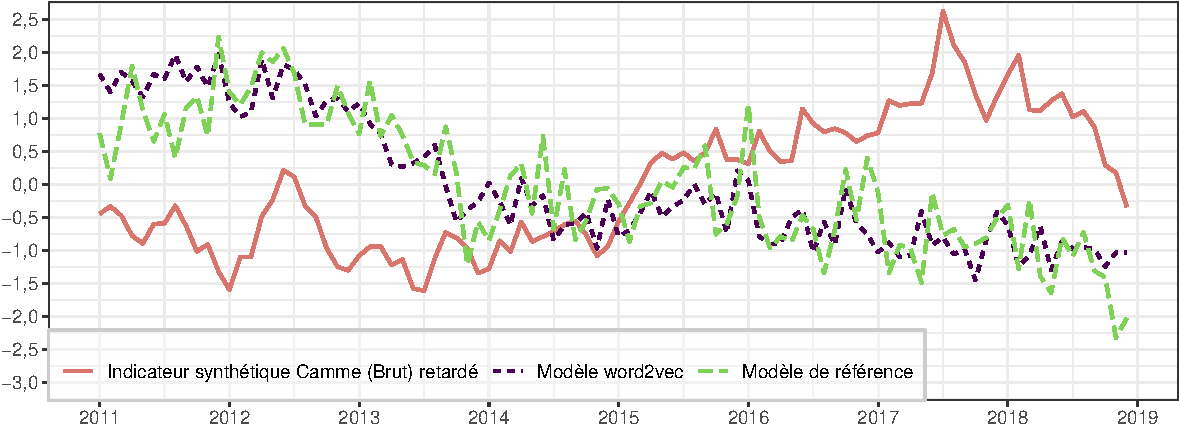
\includegraphics[width =\textwidth]{img/rmd-graphSentiments-1}}
\captionsetup{margin=0cm,format=hang,justification=justified}
\caption{Indicateur synthétique brut de confiance des ménages de l'enquête Camme (retardé) et indicateurs mensuels de sentiment construits à partir de nos modèles logit \emph{word-embedding} et lexical.}\label{fig:bslogcam}
\footnotesize
\emph{Note de lecture : tous les indicateurs sont centrés-réduits (de moyenne nulle et de variance unitaire) entre janvier 2011 et décembre 2018.}

\emph{L'indicateur Camme brut, calculé par les auteurs, est obtenu en utilisant les mêmes soldes d'opinion et coefficients que ceux de l'indicateur synthétique publié par l'Insee, mais en utilisant les soldes d'opinion bruts plutôt que CVS-CJO.
Cet indicateur est retardé : la valeur au mois $m$ correspond à la publication du mois $m+1$.}
\end{figure}

Afin de regarder les similitudes entre nos indicateurs de sentiment et
l'indicateur Camme, nous utilisons un algorithme de déformation
temporelle dynamique --- \emph{Dynamic Time Warping} (DTW) (voir par
exemple \cite{dtw} pour son implémentation en \faRProject{} que nous
utilisons ici). Cet algorithme permet de calculer une distance entre
deux séries temporelles robuste aux différences d'amplitude et aux
décalages temporels. Ainsi, la distance entre une série et la même série
retardée sera nulle (les deux séries représentent la même information)
alors que cela ne serait pas le cas si on utilisait d'autres distances,
comme la distance euclidienne. Cette méthode conclut sur le fait que la
similarité entre l'indicateur Camme et notre indicateur de sentiment
issu du modèle lexical est légèrement plus grande que celle entre
l'indicateur Camme et l'indicateur de sentiment calculé à partir du
modèle logit sur les \emph{sentence-embeddings}.

\subsubsection{Et dans une optique de prévision
?}\label{et-dans-une-optique-de-pruxe9vision}

Les deux indices de sentiments issus des tweets du mois \(m\) peuvent se
rapprocher des résultats de l'enquête Camme du mois \(m+1\) et sont
alors disponibles un mois plus tôt. Nous allons donc étudier dans quelle
mesure nos indicateurs permettent de prévoir les résultats de
l'indicateur synthétique de Camme.

Dans cette partie, afin que les résultats économétriques soient valides,
il faut que les séries soient stationnaires. La figure
\ref{fig:bslogcam} suggère la présence d'une tendance stochastique dans
tous les indicateurs (confirmée par les tests de Philipps-Perron et
KPSS), y compris lorsqu'ils sont désaisonnalisés. C'est pourquoi nous
différencions les séries désaisonnalisées pour les rendre stationnaires.

L'indicateur de sentiment issu du modèle logit sur les
\emph{sentence-embeddings} cause au sens de Granger l'indicateur
synthétique issu de l'enquête Camme (p-valeur de 0,05). C'est-à-dire que
la connaissance de l'évolution de notre second indicateur de sentiment
apporte de l'information pour prévoir l'évolution de l'indicateur
synthétique de l'enquête Camme. Ce n'est pas le cas pour le premier
indicateur calculé à partir du modèle lexical (p-valeur de 0,58).

Ainsi, l'exploitation des résultats de \emph{word2vec} permet,
contrairement au modèle lexical, de construire un indicateur de
sentiment anticipé d'un mois utile pour prévoir l'indicateur synthétique
de l'enquête Camme. En construisant un indicateur de sentiment à partir
d'un modèle logit entraîné sur la base présentée en
\ref{subsec:basegit}, nous aboutissons à des conclusions semblables pour
cette partie \ref{sec:camme}\footnote{En revanche, les mots inconnus y
  sont plus fréquents et le modèle obtenu présente de moins bons
  résultats en termes d'\emph{accuracy} à la fois sur une base test
  issue de cette base mais également provenant de la base sur les
  transports urbains.}.

\section*{Discussion et
prolongements}\label{discussion-et-prolongements}
\addcontentsline{toc}{section}{Discussion et prolongements}

Ce travail révèle que l'utilisation d'une méthode de
\emph{word-embedding} entraînée sur des tweets permet, grâce à un modèle
simple, de construire un indicateur de sentiment pouvant être comparé à
des indices d'opinion produits par des enquêtes de la statistique
publique. En comparant nos résultats à l'indicateur synthétique de
confiance des ménages produit par l'Insee, nous avons montré
qu'exploiter les représentations vectorielles des mots améliorait de
façon significative les résultats, puisque cela permet la construction
d'un indicateur de sentiment utile pour obtenir une estimation avancée
des résultats de cette enquête. Toutefois, les évolutions temporelles de
ces deux séries demeurent très différentes et nos résultats peuvent être
prolongés en de nombreux points.

La première raison de leur différence est probablement leur philosophie
distincte. Alors que l'indicateur Camme résume l'opinion des ménages sur
des sujets très spécifiques (évolution du niveau de vie, du chômage,
etc.), notre indicateur de sentiment mesure simplement la positivité /
négativité des mots employés dans des tweets, sans cibler de thématique
particulière. Or, l'opinion des Français évolue différemment en fonction
des sujets de société concernés (figure \ref{fig:figconclu}).

\begin{figure}[htp]
{\centering 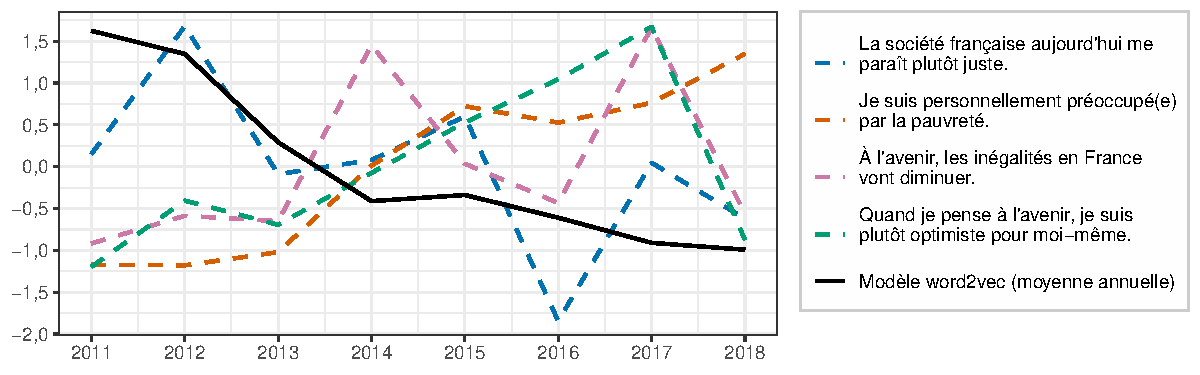
\includegraphics[width =\textwidth]{img/rmd-graphConclu-1}}
\captionsetup{margin=0cm,format=hang,justification=justified}
\caption{Opinion des Français sur les sujets sociaux et indicateur annuel de sentiment construit à partir de \emph{word2vec}.}\label{fig:figconclu}
\footnotesize
\emph{Source : Baromètre d'opinion de la DREES, 2011-2018.}

\emph{Note de lecture : tous les indicateurs sont centrés-réduits (de moyenne nulle et de variance unitaire) entre janvier 2011 et décembre 2018.}
\end{figure}

L'idéal serait de disposer d'\textbf{une base de tweets traitant de
sujets divers, et bien annotés} qui contiendrait une plus grande
gradation de sentiments (permettant notamment qu'ils soient catégorisés
de «~neutres~»). Il faudrait pour cela mobiliser un analyseur de
sentiments performant pour les tweets en français, or peu de modèles de
NLP préentraînés sont disponibles en dehors de l'anglais. Quelques
avancées récentes, comme CamemBERT (\cite{Martin}), le cousin français
de BERT entraîné sur 138 GB de texte français issu du web, pourrait par
exemple être mobilisé. L'outil BERT de Google permet en effet non
seulement de qualifier le sentiment global d'un texte mais également
d'identifier de quel sujet il traite. Une étape de sélection de données
semble en effet indispensable pour que les tweets annotés de la base
d'entraînement soient en lien avec l'enquête Camme de l'Insee. Cela
pourrait passer non seulement par l'analyse approfondie du contenu du
tweet (notamment via l'utilisation de \emph{hashtags}) mais également
son auteur (médias, faux comptes, individus lambdas\dots).

En amont de \emph{word2vec}, un \textbf{prétraitement plus approfondi
des tweets} pourrait contribuer à l'amélioration de la qualité des
vecteurs-mots et à la réduction des mots inconnus. Les mots mal
orthographiés (lettres en trop, oubli d'espace, mauvaise
ponctuation\dots) accroissent en effet considérablement la taille du
vocabulaire et la rareté des mots. Cette correction doit toutefois être
effectuée avec précaution : les différentes orthographes d'un même mot
peuvent parfois refléter des sentiments différents. Par exemple, « lol
», « LOL » et « loool » sont peut-être utilisées dans des contextes
différents : ironie, blagues, rires\dots 

Certains modèles ont montré que de considérer les mots comme étant des
séquences d'unités de sous-mots\footnote{On représente un mot non
  seulement comme lui-même mais aussi grâce à des sacs de \(n\)-grammes
  constitutifs. Si \(n = 3\), « WHERE » est représenté non seulement par
  \texttt{\textless{}where\textgreater{}} mais également
  \texttt{\textless{}wh,\ whe,\ her,\ ere,\ re\textgreater{}}.},
améliore certaines tâches d'apprentissage comme par exemple les
traductions (\cite{Sennrich}). L'extension \emph{fasttext}\footnote{La
  bibliothèque open-source \url{https://fasttext.cc/} permet de
  télécharger des modèles pré-entraînés dans 157 langues différentes.}
(\cite{Bojanowski}) de \emph{word2vec} modélise ce principe et permet
ainsi un meilleur traitement des mots rares. Il serait également
possible de gérer avec plus de précision les mots inconnus, en étudiant
leur nature et l'impact de notre méthode d'imputation sur les prévisions
de sentiments.

Enfin, l'utilisation de \textbf{modèles d'analyse de sentiment plus
élaborés}, comme les réseaux de neurones récurrents, amélioreraient
peut-être également la qualité de la prévision du sentiment d'un tweet.

\newpage

\section*{Conclusion}\label{conclusion}
\addcontentsline{toc}{section}{Conclusion}

Ce projet très riche nous a permis de partir à la découverte des
méthodes d'apprentissage par réseaux de neurones, via le modèle
\emph{word2vec}. Nous nous sommes imprégnés de son fonctionnement et
l'avons implémenté dans son ensemble grâce à la librairie
\texttt{Pytorch} de Python (partie \ref{sec:word2vec}). Au-delà de la
compréhension et de l'implémentation du modèle, nous nous sommes
également initiés aux tests d'hyperparamètres et à son évaluation sur un
corpus fictif (partie \ref{sec:evaluation}) grâce à plusieurs méthodes
(calculs de similarités cosinus, opérations vectorielles sur les mots,
méthodes de réduction de dimension ACP et t-SNE et jugement humain). Il
a été fascinant d'observer à quel point le modèle présente d'excellents
résultats en termes de capture sémantique des mots dans un texte.

Dans la partie \ref{sec:sentimentalAnalysis} dédiée à l'analyse de
sentiment, nous avons pu appliquer sur un cas concret plusieurs méthodes
étudiées durant notre deuxième année à l'ENSAE (modèles de prédiction
binaire, analyse de séries temporelles, minimisation du risque empirique
/ validation croisée\dots). L'entraînement et le test du modèle logit
dont les prédicteurs correspondent aux dimensions des
\emph{word-embeddings} nous a permis de remarquer qu'en plus de
représenter la proximité entre mots, le modèle \emph{word2vec} permet de
capter dans une certaine mesure le sentiment de phrases.

Bien sûr, la comparaison de l'indice mensuel de sentiment moyen des
tweets que nous avons construit avec l'indicateur synthétique de
confiance des ménages peut à première vue paraître «~décevante~» en
raison des différences observées entre les deux séries. Toutefois, le
test de causalité au sens de Granger nous indique que l'indice obtenu
s'avère utile pour prédire l'indicateur Camme.

La possibilité d'obtenir deux indicateurs très proches était assez
utopique en raison de leurs philosophies différentes. Au-delà de la
positivité ou négativité d'un tweet, il demeure important de déceler les
sujets sur lesquels les tweets portent pour créer un indice plus ciblé.
Par ailleurs, les bases d'entraînement et de test utilisées pour
entraîner le modèle comportent de nombreuses limites
(\emph{domain-shift}, processus d'annotation, mots inconnus).
L'identification de ces limites invite à de nombreuses pistes
d'amélioration précisées dans la partie précédente.

Les méthodes d'apprentissage étant en perpétuelle évolution, le modèle
\emph{word2vec} mis en exergue en 2013, connaît déjà des
«~concurrents~». Le plus connu est certainement \emph{GloVe} pour
«~\emph{Global Vectors}~» (\cite{Pennington}). Alors que \emph{word2vec}
privilégie l'utilisation de «~n-grammes~» (avec l'utilisation des mots
contextes qui se situent autour d'une fenêtre du mot focus),
\emph{GloVe} se base sur l'ensemble les statistiques d'occurrence des
mots du corpus (matrice de cooccurrence mot-mot) et prétend permettre
alors, par construction, de capturer des statistiques plus générales
liées au corpus.

\newpage

\appendix


\addtocontents{toc}{\protect\setcounter{tocdepth}{1}}

\section{Comment évaluer le modèle ?}\label{annexe:commentEvaluer}

\subsection{Distance entre deux mots}\label{distance-entre-deux-mots}

L'un des enjeux principaux du modèle étant de pouvoir estimer la
proximité entre deux vecteurs-mots, nous pouvons tout d'abord mesurer
cette dernière par des calculs de distance.

Il existe différents types de distances. Chacune d'elles possède des
propriétés intéressantes et s'adaptent plus ou moins bien au problème
traité. Nous avons ici retenu deux distances classiquement utilisées :

\begin{itemize}
\tightlist
\item
  \textbf{la distance euclidienne} :
  \(d_{e}(\vec{u},\vec{v}) = \left\| \vec{u} - \vec{v} \right\|_2\)\\
  Un problème est que la longueur du vecteur mot, captée dans le cas de
  la distance euclidienne, est positivement corrélée à la fréquence
  d'apparition du mot (\cite{Schakel}). Cette information peut s'avérer
  utile dans l'analyse de la signification des mots, notamment lorsque
  l'on effectue des opérations sur les vecteurs (comme l'exemple de
  \(\overrightarrow{Paris} - \overrightarrow{France} + \overrightarrow{Italie} = \overrightarrow{Rome}\)
  dans \cite{Mikolov}).\\
  Toutefois, cette dépendance à la fréquence d'apparition peut également
  fausser l'analyse. C'est pourquoi il est utile de normaliser les
  vecteurs :
  \[ d_{e}(\vec{u},\vec{v}) = \left\| \frac{\vec{u}}{\left\| \vec{u} \right\|_2} - \frac{\vec{v}}{\left\| \vec{v} \right\|_2}  \right\|_2\]
\item
  \textbf{la similarité cosinus} :
  \(d_{c}(\vec{u}, \vec{v}) = \frac{\vec{u}.\vec{v}}{\left\| \vec{u} \right\|_2 \left\| \vec{v} \right\|_2 }\).\\
  La similarité cosinus correspond au produit scalaire entre les deux
  vecteurs normalisés. Elle mesure ainsi l'angle formé entre deux
  vecteurs-mots.\\
  C'est la distance que de nombreux papiers fondateurs de la méthode
  \emph{word2vec} (comme \cite{Mikolov} ou \cite{Levy}) utilisent, avec
  l'argument selon lequel les mots apparaissant dans des contextes
  similaires sont groupés dans la même direction durant l'entraînement.
  Une similarité est proche de \(+1\) si deux mots sont positivement
  reliés (proches), de \(-1\) s'ils sont négativement reliés (éloignés)
  et de 0 s'ils ne sont pas \og reliés \fg{}.\\
  Il est toutefois délicat d'interpréter une similarité proche de
  \(-1\). On pourrait intuitivement penser à des antonymes, comme
  \og grand \fg{} et \og petit \fg{}, mais en pratique, les antonymes
  sont susceptibles d'apparaître dans des contextes semblables et sont
  donc bien souvent positivement corrélés.
\end{itemize}

\subsection{Analyse en Composantes
Principales}\label{analyse-en-composantes-principales}

Une fois le modèle \emph{word2vec} entraîné, nous obtenons des
\emph{word-embeddings} pour chacun de nos mots, représentés par des
vecteurs de grandes dimensions (20, 50 ou même supérieures à 100).

Dès lors, il devient complexe de bien observer la proximité entre deux
mots. C'est pourquoi il devient utile de mobiliser des méthodes de
réduction de dimensions comme l'analyse en composantes principales
(ACP). En effet, l'objectif premier de cette méthode est de projeter un
nuage de points sur un espace de dimension inférieure. Cela permet de
rendre l'information moins redondante et plus visuelle, tout en étant le
plus proche possible de la réalité.

Considérons le cas où nous disposons de \(n\) individus (dans notre cas
les mots) et de \(p\) variables (dans notre cas, leurs composantes ou
dimensions issues du modèle \emph{word2vec}). On note \(X = (x_{ij})\)
la matrice de taille \((n,p)\) des données brutes, où \(x_{ij}\)
représente la valeur de la \(j\)-ème variable pour le \(i\)-ème
individu. Mathématiquement, pour définir l'ACP, on définit deux espaces
:

\begin{itemize}
\item
  L'\emph{espace des individus}, de dimension \(p\), auquel on associe
  la métrique \(M\) utilisée pour le produit scalaire. Dans la suite
  nous utiliserons \(M =I_p\) la matrice identité. La norme et le
  produit scalaire associés à \(M\) sont donc euclidiens.
\item
  L'\emph{espace des variables}, de dimension \(n\), auquel on associe
  la métrique \(N=diag(p_1,...,p_n)\) avec \(\sum_{i=1}^np_i=1\). La
  matrice \(N\) représente le poids donné à chaque individu. Par
  simplification, nous utiliserons ici des poids uniformes :
  \(N=\frac{1}{n}I_n\). Afin de donner le même poids à toutes les
  variables, chaque variable est centrée-réduite : cela revient à
  centrer-réduire les colonnes de notre matrice \(X\). Nous notons
  \(Z =\bar X= (z_{ij})\) la matrice des données centrées et
  réduites\footnote{Nous travaillons ici dans le cadre d'une ACP normée
    où la matrice \(X\) a été centrée puis réduite. La réduction de
    \(X\) a modifié les distances initiales entre individus
    (\(\langle z_i,z_{i'}\rangle_M \neq \langle x_i,x_{i'}\rangle_M\)).
    Cela n'aurait pas été le cas si la matrice \(X\) avait été
    uniquement centrée (ACP non normée).}.
\end{itemize}

Pour toute métrique \(D\) (\(D=N\) ou \(D=M\)), on associe le produit
scalaire \(\langle x,y\rangle_{D} = {}^t\!xD y\). La construction des
axes de l'ACP est faite par projection orthogonale. La projection
orthogonale d'un individu \(i\) (vecteur ligne) \(z_i\) sur une droite
de vecteur directeur unitaire \(v\) vaut
\(\langle {}^tz_i,v\rangle_{M}=z_i\times v\) et les coordonnées de
projection des \(n\) individus valent \(Zv\).

Les vecteurs directeurs des axes sont définis de manière à maximiser la
dispersion du nuage (son inertie\footnote{La dispersion d'un nuage de
  points unidimensionnel par rapport à sa moyenne se mesure par la
  variance. Dans le cadre multidimensionnel, la dispersion du nuage par
  rapport à son barycentre \(\bar z\) se mesure par l'inertie, qui
  généralise la variance.}) des individus projetés et conserver ainsi au
mieux les distances entre les individus. L'inertie se définit alors
comme :

\begin{align*}
I(Z) &= \sum_{i = 1}^n p_i\|z_i-\bar{z}\|_M^2 \text{ avec }
  \bar{z} = 
  \begin{pmatrix}\bar z_{1} \\
    \vdots \\ \bar z_{p}
  \end{pmatrix} =
  \begin{pmatrix}\frac 1 n \sum_{i=1}^n z_{i,1} \\
    \vdots \\ \frac 1 n \sum_{i=1}^n z_{i,p}
  \end{pmatrix} (= 0_{\mathbb R^p}\text{ dans notre cas})
\\&=\sum_{i = 1}^n \frac 1 n \sum_{j=1}^p (z_{i,j} -  \bar{z}_j)^2  \text{ car }M=I_p 
\\&=\sum_{j = 1}^p \frac 1 n \sum_{i=1}^n (z_{i,j} -  \bar{z}_j)^2
\\&=\sum_{j = 1}^p Var(z^j)\text{, avec } z^j = 
  \begin{pmatrix} z_{1,j} \\ \vdots \\  z_{n,j} 
  \end{pmatrix}
\\ &= p \text{ car les variables sont réduites}
\end{align*}

On trouve tout d'abord le vecteur directeur \(v_1\) qui orientera le
premier axe de l'ACP grâce au programme suivant : \[
v_1 =\underset{\| v \|_M = 1}{\mathrm{argmax~}} 
\underbrace{\|Zv\|_N}_{=Var(Zv)} =\underset{\| v \|_M = 1}{\mathrm{argmax~}} ^t\!vR v 
\] où \(R = Var(Z) = \frac{1}{n} ^t\!Z Z\) est la matrice des
corrélations entre les \(p\) variables.

Puis, on choisit \(v_2\) orthogonal à \(v_1\) tel que l'inertie soit
toujours maximisée : \[
v_2 =\underset{ \| v \|_M = 1,\,v \perp v_1}{\mathrm{argmax}}\;  Var(Zv)
\] En procédant de manière séquentielle, on obtient \(q < r\) axes
orthogonaux avec \(r = rg(Z)\) et \(q\) choisi par le
statisticien\footnote{Différentes méthodes existent afin de déterminer
  le \(q\) optimal, comme la règle de Kaiser ou encore celle du coude.}.

On peut montrer que \(\forall k < q\) :

\begin{itemize}
\tightlist
\item
  \(v_k\) est un vecteur propre associé à la k\ieme{} valeur propre
  \(\lambda_k\) de \(R\) (les valeurs propres étant rangées par ordre
  décroissant) ;
\item
  la composante principale \(Zv_k\) est centrée et
  \(V(Zv_k)= \lambda_k\) ;
\item
  les \(Zv_k\) ne sont pas corrélés entre eux.
\end{itemize}

On obtient alors la matrice \(F = ZV\) des nouvelles coordonnées
factorielles des individus, avec \(V = (v_1,\dots,v_q)\) la matrice des
vecteurs propres. Nous utilisons ici l'ACP en vue d'identifier les
individus (ici, nos mots) qui sont proches. Pour ce faire, il suffit de
représenter les coordonnées factorielles de la matrice \(F\) dans des
repères, en général en deux dimensions pour une question de lisibilité.
Deux mots apparaissant dans des contextes similaires seront proches sur
ce repère et orientés dans la même direction.

\subsection{\texorpdfstring{Algorithme \emph{t-distributed Stochastic
Neighbor
Embedding}}{Algorithme t-distributed Stochastic Neighbor Embedding}}\label{algorithme-t-distributed-stochastic-neighbor-embedding}

Bien que l'ACP soit une première manière de résumer l'information
contenue dans nos vecteurs, elle présente des limites, notamment dans
les vecteurs aux trop grandes dimensions, pour lesquels l'inertie des
premiers axes de l'ACP peut se révéler faible.

Pour combler ces lacunes, un autre algorithme de réduction de dimension
peut être utilisé, celui dit du \emph{t-distributed Stochastic Neighbor
Embedding} (t-SNE). Contrairement à l'ACP, cet algorithme est
stochastique et non-linéaire et il favorise l'apparition de groupes de
mots proches. Sa philosophie demeure cependant identique : représenter
dans un espace à dimension réduite notre nuage de points de manière à
repérer les mots proches.

La première étape de l'algorithme consiste à calculer les similarités
entre les \(n\) vecteurs-mots \((x_i)_{i=1...n}\). La similarité entre
\(x_i\) et \(x_j\) se mesure comme étant la probabilité conditionnelle
\(p_{j|i}\) de choisir \(x_j\) comme voisin de \(x_i\), si les voisins
étaient tirés au sort selon une loi
\(\mathcal{N}(x_i, \sigma_i)\)\footnote{\(\sigma_i\) doit être calculé
  de manière à adapter la loi conditionnelle aux données. Une faible
  dispersion autour de \(x_i\) entraînera un \(\sigma_i\) faible et
  réciproquement. Il s'agit de trouver le \(\sigma_i\) qui minimise ce
  qui est appelé en théorie de l'information la \og perplexité \fg{},
  c'est-à-dire un indicateur qui décrit à quel point une distribution de
  probabilité réussit à prédire un échantillon.} :

\[ p_{j|i} = \frac{
\exp\left(-\frac{(d_e(x_i - x_j))^2}{2\sigma_i^2}\right)
}{
\sum_{k \neq i}
\exp\left(-\frac{(d_e(x_i - x_k))^2}{2\sigma_i^2}\right)
}\]

La seconde étape de l'algorithme consiste à trouver le nouvel espace de
projection à faible nombre de dimensions. On appellera \(g_i\) les
\(x_i\) projetés dans cet espace que l'on cherche à déterminer. On
calcule maintenant les probabilité conditionnelles \(q_{j|i}\) de
choisir \(g_j\) comme voisin de \(g_i\) en supposant que les \((g_i)_i\)
suivent cette fois-ci une distribution de \emph{Student} --- d'où le nom
de l'algorithme --- plutôt qu'une loi gaussienne\footnote{Dans un espace
  à faible dimension, la dispersion des vecteurs est réduite. La
  distribution de Student possède des queues plus épaisses que la loi
  normale, ce qui permet de mieux différencier les vecteurs distants des
  vecteurs similaires.}.

\[ q_{j|i} = \frac{(1+ (d_e(g_i - g_j))^2)^{-1}}{\sum_{k \neq i}{(1+ (d_e(g_i - g_k))^2)^{-1}}}\]

Afin d'obtenir les \(g_i\), on minimise, par descente de gradient, la
divergence de Kullback--Leibler entre les distributions de probabilité P
et Q des \(p_{ij}\) et \(q_{ij}\) définie par :
\[KL(P,Q) = \sum_{i \neq j} { p_{ij} \log{\frac{p_{ij}}{q_{ij}}}} \qquad\text{avec}\qquad p_{ij} = \frac{p_{i|j} + p_{j|i}}{2n}\]

Comme dans l'algorithme de l'ACP, l'algorithme de t-SNE nous permet
d'obtenir une nouvelle projection des \(x_i\). Il faut cependant
analyser avec précaution ses résultats. L'algorithme n'étant pas
linéaire, l'interprétation de la taille des \emph{clusters} obtenus ou
de la distance qui les sépare n'est alors pas directe.

\subsubsection{Jugement humain}\label{sec:jugementHumain}

Les \emph{word-embeddings} obtenus par \emph{word2vec} sont censés
regrouper les mots qui apparaissent dans un contexte similaire. Une
dernière façon de vérifier la qualité de nos vecteurs-mots est de les
comparer à un jugement humain. Pour ce faire, nous utilisons la liste de
référence RG-65 pour le français\footnote{Le RG-65 a fait appel à 18
  évaluateurs humains. La base, initialement mobilisée dans un article
  anglophone (\cite{Rubenstein}) a été traduite de l'anglais.}
(\cite{Boumedyen}). Elle contient 65 paires de noms communs (tableau
\ref{table:human_judgement}) évaluées sur une échelle de 0 (non liés) à
4 (très liés).

\begin{table}[!h]
\begin{center}
\begin{tabular}{|c|c|c|}
    \hline
    mot 1 & mot 2 & similarité  \tabularnewline
    \hline
    corde & sourire & 0,00   \tabularnewline
    midi & ficelle & 0,00   \tabularnewline
    $\vdots$  & $\vdots$  & $\vdots$    \tabularnewline
    corde & ficelle & 3,33   \tabularnewline
    $\vdots$  & $\vdots$  & $\vdots$    \tabularnewline
    automobile & auto & 3,94   \tabularnewline
    coq & coq & 4,00   \tabularnewline
    \hline
 \end{tabular}
\captionsetup{margin=0cm,format=hang,justification=justified}
\caption{Base de données de jugement humain.}\label{table:human_judgement}
\end{center}
\end{table}

Nous calculons ensuite la corrélation de Spearman entre les similarités
cosinus de ces différentes paires issues de notre modèle (notées ici
\((X_i)_{i=1..n}\)) et les scores proposés ci-dessus par des êtres
humains (notés ici \((Y_i)_{i=1..n}\)).

La corrélation de Spearman est égale au coefficient de corrélation de
Pearson calculé sur les variables de rang. \[
r_s = \mathrm{corr}(\mathrm{rg}_X, \mathrm{rg}_Y) = 
\frac{\mathrm{cov}(\mathrm{rg}_X, \mathrm{rg}_Y)}{
\sigma_{\mathrm{rg}_X} \sigma_{\mathrm{rg}_Y}
}
\] La variable de rang \(\mathrm{rg}_{X_i}\) est définie telle que
\(\mathrm{rg}_{X_i}=j \iff X_i = X_{(j)}\) (\(X_i\) est la \(j\)ème plus
petite variable).

Pour tester la significativité de ce coefficient, nous utilisons la loi
sous \((H_0)\) de la statistique de test
\(z = \arctanh(r_s) = \frac{1}{2} \ln\frac{1+r}{1-r} \overset{H_0}{\sim}\mathcal{N}(0, \frac{1}{n-3})\)
et obtenons l'intervalle de confiance suivant :

\[
IC_\alpha (r_s) = \left[\tanh\left(z-\frac{q_{1-\frac{\alpha}{2}}}{\sqrt{n-3}}\right),
\tanh\left(z+\frac{q_{1-\frac{\alpha}{2}}}{\sqrt{n-3}}\right)\right]
\] avec \(q_{1-\frac{\alpha}{2}}\) le quantile d'ordre
\(1-\frac{\alpha}{2}\) d'une loi \(\mathcal{N}(0, 1)\).

\newpage

\section{Correction des effets saisonniers et jours
ouvrables}\label{annexe:cvscjo}

La figure \ref{fig:cvscjo} compare les séries brutes et corrigées des
variations saisonnières et des jours ouvrables (CVS-CJO) des trois
indicateurs étudiés. Même si les séries brutes semblent très proches des
séries désaisonnalisées, la présence de saisonnalité est confirmée par
le F-test proposé par \cite{lytras}.

Dans cette annexe, nous présentons la manière dont nous désaisonnalisons
nos deux indicateurs de sentiment calculés à partir des tweets. Pour
rappel, l'indicateur synthétique de confiance des ménages publié par
l'Insee grâce à l'enquête Camme est calculé à partir de soldes d'opinion
CVS-CJO, c'est pourquoi on considère ici qu'il est CVS-CJO. L'indicateur
brut associé correspond à l'indicateur que l'on obtient en utilisant les
mêmes soldes d'opinion et les mêmes coefficients que dans l'indicateur
publié par l'Insee mais en utilisant les soldes d'opinion bruts plutôt
que CVS-CJO.

\begin{figure}[htp]
{\centering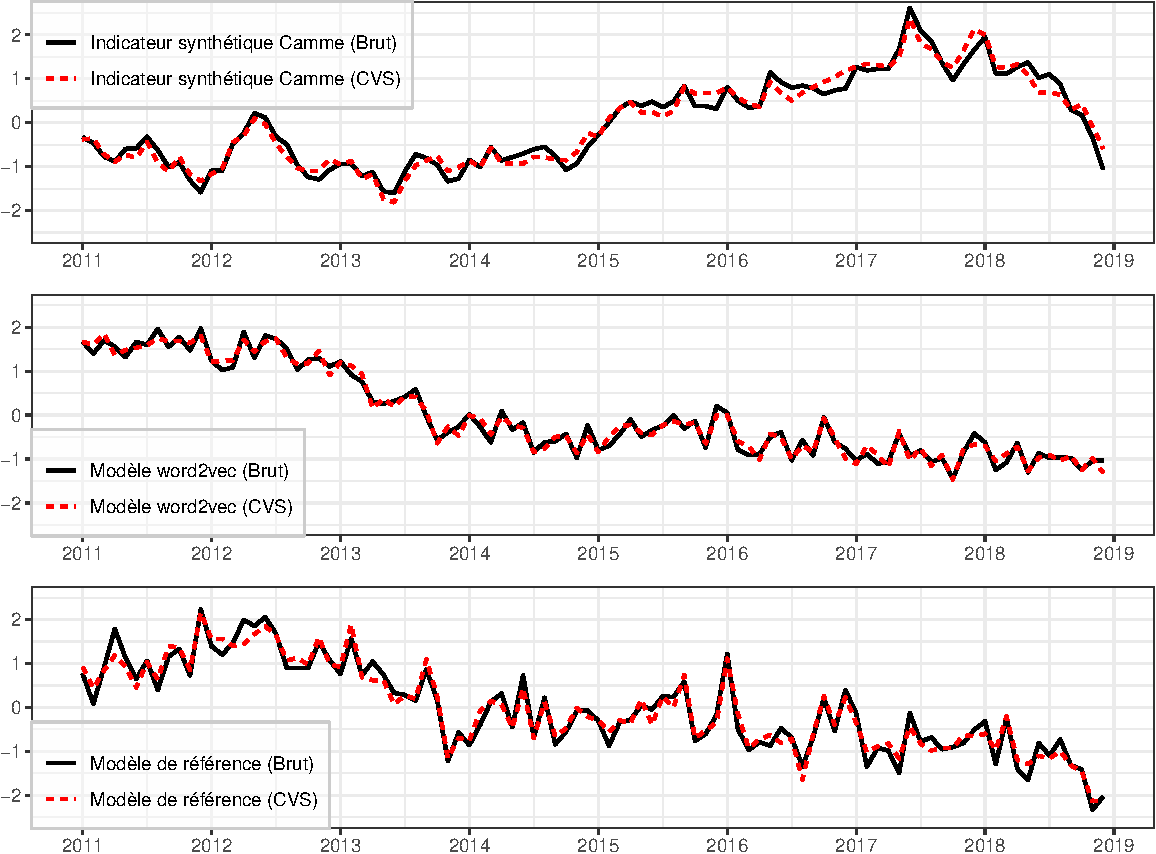
\includegraphics[width = \textwidth]{img/rmd-graphCVS-1}}
\captionsetup{margin=0cm,format=hang,justification=justified}
\caption{Comparaison des séries brutes et CVS-CJO de l'indicateur synthétique de confiance des ménages de l'enquête Camme et des indicateurs mensuels de sentiment que nous avons construits à partir des modèles logit et lexical.}\label{fig:cvscjo}
\footnotesize

\emph{L'indicateur Camme brut correspond à l'indicateur que l'on obtient en utilisant les mêmes soldes d'opinion et les mêmes coefficients que dans l'indicateur synthétique publié par l'Insee mais en utilisant les soldes d'opinion bruts plutôt que CVS-CJO.}

\emph{Les autres indicateurs ont été corrigés des variations saisonnières et des jours ouvrables (CVS-CJO) par la méthode X-12ARIMA.}
\end{figure}

Pour désaisonnaliser nos deux indicateurs de sentiment, nous avons
utilisé la méthode X-12ARIMA qui fonctionne en deux étapes :

\begin{enumerate}
\def\labelenumi{\arabic{enumi}.}
\item
  La série initiale est pré-ajustée de certains effets déterministes
  (effets jours ouvrables et points atypiques) grâce à un modèle de
  régression linéaire dont les résidus suivent un modèle ARIMA (partie
  \ref{sec:cjo}).
\item
  Cette série pré-ajustée est ensuite désaisonnalisée par une méthode
  non-paramétrique qui repose sur l'usage de moyennes mobiles (partie
  \ref{sec:cvs}).
\end{enumerate}

\subsection{Correction des effets jours ouvrables}\label{sec:cjo}

Dans la correction des effets saisonniers et des effets jours ouvrables
(CVS-CJO), on distingue trois types d'effets :

\begin{itemize}
\item
  un effet \emph{nombre de jours} lié au nombre de jours dans le mois ;
\item
  un effet \emph{type de jour} lié au nombre de jours de chaque type
  (lundi, mardi\dots) ;
\item
  un effet \emph{fêtes mobiles} lié à la variation d'une année sur
  l'autre de la date de certaines fêtes comme Pâques.
\end{itemize}

Dans notre cas, puisque les tweets sont tirés à des jours fixes, il n'y
a pas d'effet nombre de jours et l'effet fête mobile n'aurait pas de
sens. En revanche, il pourrait y avoir un effet type de jour : on peut
par exemple supposer que les thèmes traités par les tweets, et donc les
sentiments, sont différents en fonction du jour de la semaine. Les
sentiments exprimés par les tweets pourraient donc être influencés par
les types de jours échantillonnés pour tirer aléatoirement les tweets.

Pour estimer l'effet jour ouvrable, nous utilisons l'approche de la
méthode X-12ARIMA, notamment décrite dans \cite{L2018}.

Supposons que le \(j\)\textsuperscript{ème} jour de la semaine a un
effet \(\alpha_j\) où \(j=1\) désigne le lundi, \(j=2\) le mardi, \dots,
et \(j=7\) le dimanche. Chaque \(\alpha_j\) représente par exemple le
sentiment moyen d'un jour \(j\). Si \(N_{jt}\) représente le nombre de
jours \(j\) dans le mois \(t\), la longueur du mois \(t\) est alors
\(N_t = \sum_{j=1}^{7} N_{jt}\) et l'effet cumulé pour ce mois (le
sentiment moyen du mois) sera : \[
TD_t = \sum_{j=1}^{7} \alpha_j N_{jt}
\]

Une première idée pour détecter et évaluer les effets de jours ouvrables
dans une série est d'expliquer les valeurs de la série par les 7
variables \(N_{jt}\). Mais ces régresseurs sont par nature saisonniers
(il y a en moyenne plus de lundis en janvier qu'en février) et fortement
corrélés.

Une formulation différente mais équivalente de l'effet jours ouvrables
permet de résoudre en grande partie ces problèmes. L'effet journalier
moyen, l'opinion moyenne sur une journée, s'écrit
\(\bar{\alpha} = \sum_{j=1}^7 \alpha_j /7\). Comme par construction
\(\sum_{j=1}^7 \left(\alpha_j-\bar{\alpha}\right) = 0\), on peut écrire
:

\begin{eqnarray*}
\sum_{j=1}^7 \alpha_j N_{jt} & = & \bar{\alpha}N_t + \sum_{j=1}^7 \left(\alpha_j-\bar{\alpha}\right) N_{jt} \nonumber \\
& = &  \bar{\alpha}N_t + \sum_{j=1}^6 \left(\alpha_j-\bar{\alpha}\right) \left(N_{jt} - N_{7t}\right).
\end{eqnarray*}

Ainsi, l'effet cumulatif du mois se décompose en un effet directement
lié à la longueur du mois et un effet net de chaque jour de la semaine.
Comme la quantité \(\bar{\alpha}N_t\) est par nature saisonnière
(janvier a toujours plus de jours que février), on utilise en fait
l'égalité :
\(\bar{\alpha}N_t = \bar{\alpha}N_t^* + \bar{\alpha}\left(N_t-N_t^*\right)\),
où \(N_t^*\) représente la moyenne de la longueur du mois \(t\). En
d'autres termes, \(N_t^*\) est égal à \(30\) ou \(31\) si le mois
considéré n'est pas un mois de février et à \(28,25\) dans le cas
contraire. Le second terme de l'égalité est donc nul sauf pour le mois
de février. L'utilisation des variables contrastes (considérer
\(N_{7t}\) comme variable de référence) permet donc de désaisonnaliser
les régresseurs jours ouvrables.

La version actuelle de X-12ARIMA utilise le modèle Reg-ARIMA suivant
pour estimer les effets de jours ouvrables :

\begin{equation}
y_t=\beta_0 LY_t + \sum_{j=1}^{6} \beta_j \left(N_{jt} - N_{7t}\right) + \varepsilon_t
    \label{eq:eqcjotd}
\end{equation}

où \(\varepsilon_t\) suit un modèle ARIMA et \(LY_t\) désigne le
régresseur « année bissextile » --- \emph{Leap Year} (LY) --- égal à :
\[
LY_{t} = \left\{ \begin{array}{rl} 
                0,75 & \mbox{si } t \mbox{ est un mois de février bissextil } \\
                -0,25 & \mbox{si } t \mbox{ est un mois de février non bissextil } \\
                0 & \mbox{sinon}
               \end{array}
         \right.
\]

Une spécification alternative consiste à regrouper les régresseurs du
lundi au vendredi et ceux du samedi et du dimanche\footnote{On a donc
  \(\beta_1=\beta_2=\dots=\beta_5\) et \(\beta_6 = 0\).}. On considère
ainsi que l'effet d'un lundi est le même que l'effet d'un mardi, etc.
jusqu'au vendredi et que cet effet est différent le samedi et le
dimanche (week-end). Le modèle \eqref{eq:eqcjotd} devient :

\begin{eqnarray}
y_t=\beta_0 LY_t + \tilde\beta_1 \left(\sum_{j=1}^{5}N_{jt} - (N_{6t} + N_{7t})\right) + \varepsilon'_t
\label{eq:eqcjowd}
\end{eqnarray}

Dans notre cas, puisqu'il n'y a pas d'effet longueur du mois nous
omettons le régresseur \(LY_t\) dans \eqref{eq:eqcjotd} et
\eqref{eq:eqcjowd}. On considère qu'il y a un effet jours ouvrables
significatif lorsque \(\exists i\in \{1,2,\dots,6\}\::\:\beta_i\ne0\) ou
lorsque \(\tilde\beta_1\ne0\).

\faArrowCircleRight{} Pour nos indicateurs de sentiment (construits à
partir des modèles logit et lexical), nous ne détectons pas d'effet
jours ouvrables. Cela ne signifie pas pour autant que le type de jour
n'a pas d'effet sur nos indicateurs de sentiment, mais que nous
n'arrivons pas à en estimer un. Cela peut venir de la méthode de
collecte : tirer les tweets tous les 1, 5, 10, 15, 20, 25 et 28 de
chaque mois revient à tirer tous les jours de la semaine sauf
un\footnote{Si le premier jour du mois est un lundi alors, parmi les 4
  200 tweets, 1 200 sont tirés un lundi, 0 le mardi et 600 les autres
  jours de la semaine.}. On peut donc difficilement isoler l'effet du
type de jour. Pour le faire, il faudrait faire une analyse plus
approfondie en construisant par exemple un indicateur de sentiment par
jour de la semaine.

\subsection{Correction des effets saisonniers}\label{sec:cvs}

L'objectif de la désaisonnalisation est de décomposer une série \(X_t\)
en trois composantes inobservées :

\begin{itemize}
\item
  \(TC_t\) la tendance-cycle : combinaison de la tendance et du cycle ;
\item
  \(S_t\) la saisonnalité : une fluctuation qui se répète d'année en
  année à la même période ;
\item
  \(I_t\) l'irrégulier : une fluctuation résiduelle non comprise dans
  les deux composantes précédentes (chocs ponctuels, etc.).
\end{itemize}

Ces composantes sont combinées entre elles selon un \emph{schéma de
composition} dont les plus classiques sont :

\begin{itemize}
\item
  le schéma additif : \(X_t=TC_t+S_t+I_t\) ;
\item
  le schéma multiplicatif \(X_t=TC_t\times S_t\times I_t\).
\end{itemize}

À partir de l'estimation de ces composantes, il est possible de
désaisonnaliser les séries en enlevant la composante saisonnière
\(S_t\).

Pour effectuer la désaisonnalisation, la méthode X-12ARIMA utilise
l'algorithme X-11. En quelques mots, c'est un algorithme qui repose sur
l'utilisation de moyennes mobiles afin d'estimer itérativement les
différentes composantes.

Le graphique \ref{fig:coefcvscjo} trace l'évolution des coefficients
saisonniers pour nos indicateurs de sentiment. L'évolution des
coefficients saisonniers de l'indicateur de sentiment calculé à partir
du modèle lexical suggère que la saisonnalité de cette série est faible.
L'étude de ceux de l'indicateur calculé à partir du modèle
\emph{word2vec} suggère que les tweets sont globalement plus pessimistes
en février et mars, et plus optimistes en avril, août et décembre.

\begin{figure}[htp]
{\centering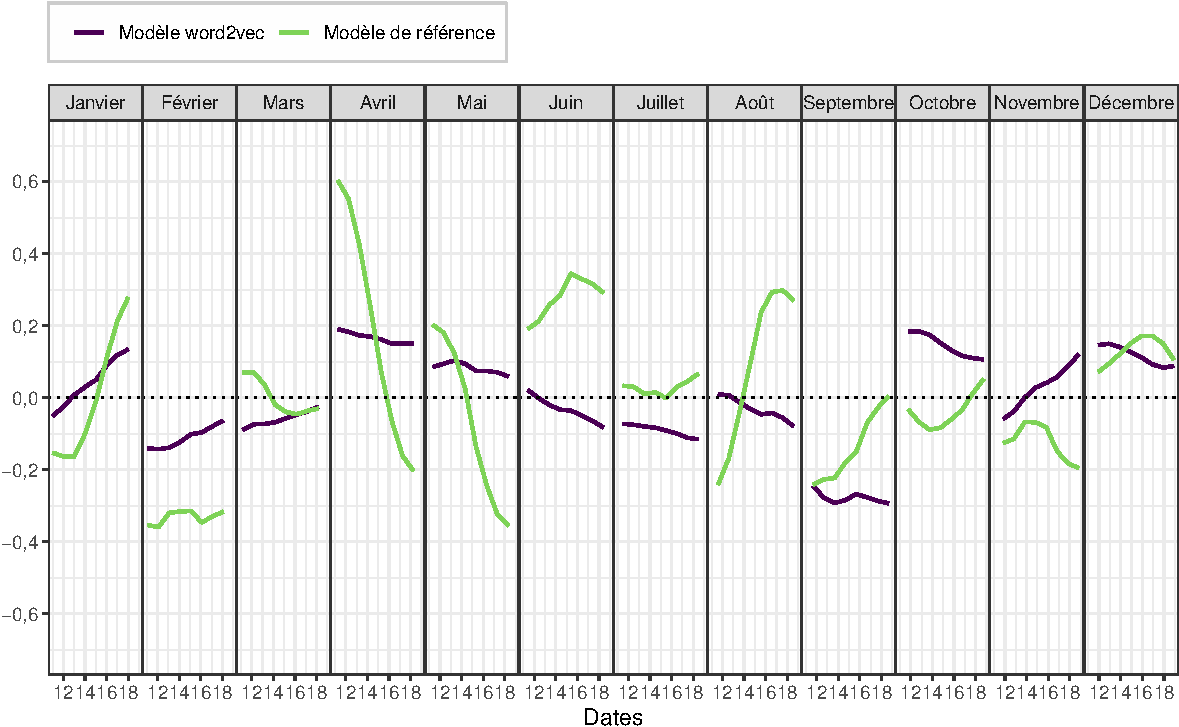
\includegraphics[width = \textwidth]{img/rmd-graphCoefCVS-1}}
\captionsetup{margin=0cm,format=hang,justification=justified}
\caption{Composantes saisonnières des indicateurs mensuels de sentiment que nous avons construits à partir de nos deux modèles (logit et lexical).}\label{fig:coefcvscjo}
\footnotesize

\emph{La composante saisonnière a été estimée par la méthode X-12ARIMA.}
\end{figure}

\newpage

\footnotesize

\nocite{*}

\begin{thebibliography}{999}
\bibitem[Bengio \emph{et al} (2003)]{Bengio} Bengio, Y., Ducharme, R., Vincent, P., Janvin, C. (2003). A Neural Probabilistic Language Model. JMLR, 3:1137–1155. \url{https://papers.nips.cc/paper/1839-a-neural-probabilistic-language-model.pdf}.
\bibitem[Bojanowski et al. (2017)]{Bojanowski} Bojanowski, P., Grave, E., Joulin, A., \& Mikolov, T. (2017). Enriching word vectors with subword information. Transactions of the Association for Computational Linguistics, 5, 135-146. \url{https://www.mitpressjournals.org/doi/abs/10.1162/tacl_a_00051}.
\bibitem[Boumedyen Billami \& Gala (2017)]{Boumedyen} Boumedyen Billami, M., Gala, N (2017). Création et validation de signatures sémantiques : application à la mesure de similarité sémantique et à la substitution lexicale. TALN 2017. \url{https://hal.archives-ouvertes.fr/hal-01528117/document}.
\bibitem[Candela et al. (2009)]{Candela} Candela, J. Q., Sugiyama, M., Schwaighofer, A., \& Lawrence, N. D. (2009) Dataset shift in machine learning. The MIT Press, 1, 5. \url{http://www.acad.bg/ebook/ml/The.MIT.Press.Dataset.Shift.in.Machine.Learning.Feb.2009.eBook-DDU.pdf}.
\bibitem[Hutter, Hoos \& Leyton-Brown (2014)]{Hutter} Hutter, F., Hoos, H., Leyton-Brown, K., (2014). An Efficient Approach for Assessing Hyperparameter Importance. PMLR 32(1):754-762. \url{http://proceedings.mlr.press/v32/hutter14.pdf}.
\bibitem[Jurafsky \& Martin (2019)]{Jurafsky} Jurafsky, D., Martin, J. H. (2019). Speech and Language Processing (3rd ed. draft). Prentice Hall. \url{https://web.stanford.edu/~jurafsky/slp3/edbook_oct162019.pdf}.
\bibitem[Ladiray (2018)]{L2018} Ladiray, D. (2018), Calendar effects, in Handbook on Seasonal Adjustment, edited by G. L. Mazzi, co-edited by D. Ladiray, European Union, Luxembourg. \url{ec.europa.eu/eurostat/web/products-manuals-and-guidelines/-/KS-GQ-18-001}.
\bibitem[Levy \& Golberg (2015)]{Levy} Levy, O., Golberg, Y. (2015). Neural Word Embedding as Implicit Matrix Factorization.
\url{https://papers.nips.cc/paper/5477-neural-word-embedding-as-implicit-matrix-factorization.pdf}.
\bibitem[Levy \& Golberg (2014)]{Levy2} Levy, O., Golberg, Y. (2014). Dependency-based word embeddings. ACL. \url{http://papers.nips.cc/paper/5477-neural-word-embedding-as-implicit-matrix-factorization.pdf}.
\bibitem[Lytras \emph{et al} (2007)]{lytras} Lytras, D. P., Feldpausch, R. M., Bell, W. R (2007). Determining Seasonality: A Comparison of Diagnostics from X-12-ARIMA, U.S. Census Bureau, presented at ICES III, June, 2007. \url{https://www.census.gov/ts/papers/ices2007dpl.pdf}.
\bibitem[Martin et al. (2019)]{Martin} Martin, L., Muller, B., Suárez, P. J. O., Dupont, Y., Romary, L., de la Clergerie, É. V., \& Sagot, B. (2019). CamemBERT: a Tasty French Language Model. arXiv preprint arXiv:1911.03894. \url{https://arxiv.org/abs/1911.03894}.
\bibitem[Mikolov \emph{et al} (2013a)]{Mikolov} Mikolov, T., Chen, K., Corrado, G., Dean, J. (2013a). Efficient Estimation of Word Representations in Vector Space. arXiv:1301.3781. \url{https://arxiv.org/pdf/1301.3781.pdf}.
\bibitem[Mikolov \emph{et al} (2013b)]{MikolovNS} Mikolov, T., Sutskever, I., Chen, K., Corrado, G. S., and Dean, J. (2013b). Distributed representations of words and phrases and their compositionality, arXiv:1310.4546. \url{https://arxiv.org/pdf/1310.4546.pdf}.
\bibitem[Pennington, Socher \& Manning (2014)]{Pennington} Pennington, J., Socher, R., Manning, C. D., (2014).  Glove: global vectors for word representation. Proc. of EMNLP,1532 – 1543. \url{https://www.aclweb.org/anthology/D14-1162.pdf}.
\bibitem[{\v R}eh{\r u}{\v r}ek \& Sojka (2010)]{Rehurek} {\v R}eh{\r u}{\v r}ek, R., Sojka, P. (2010). Software Framework for Topic Modelling with Large Corpora. Proceedings of LREC 2010 workshop New Challenges for NLP Frameworks. p. 46--50, 5 pp. ISBN 2-9517408-6-7. \url{https://is.muni.cz/publication/884893/en}.
\bibitem[Rubenstein \& Goodenough (1965)]{Rubenstein} Rubenstein, H., Goodenough, J. B. (1965). Contextual Correlates of Synonymy. Commun. ACM, 8 (10), 627–633. \url{https://dl.acm.org/doi/10.1145/365628.365657}.
\bibitem[Schakel \& Wilson (2015)]{Schakel} Schakel, A. M., Wilson, B. J. (2015). Measuring Word Significance using Distributed Representations of Words. arXiv:1508.02297. \url{https://arxiv.org/pdf/1508.02297v1.pdf}.
\bibitem[Sennrich, Haddow \& Birch (2015)]{Sennrich} Sennrich, R., Haddow, B., \& Birch, A. (2015). Neural machine translation of rare words with subword units. arXiv preprint arXiv:1508.07909. \url{https://arxiv.org/pdf/1508.07909.pdf}.
\bibitem[Tormene \emph{et al} (2008)]{dtw} Tormene P, Giorgino T, Quaglini S, Stefanelli M (2008). “Matching
Incomplete Time Series with Dynamic Time Warping: An Algorithm and an Application to Post-Stroke Rehabilitation.” \emph{Artificial Intelligence
in Medicine}, \textbf{45}(1), 11-34. doi: 10.1016/j.artmed.2008.11.007, \url{https://doi.org/10.1016/j.artmed.2008.11.007}.
\end{thebibliography}

\end{document}
